\documentclass[authoryear]{elsarticle}

	\usepackage{epsfig}
	\usepackage{bm}
	\usepackage{epstopdf}
	\usepackage{amssymb}
	\usepackage[left=2.5cm, right=2.5cm,top=4cm, bottom=4cm]{geometry}

	\newcommand{\sectionX}[1]{\section{#1}}
	\newcommand{\subsectionX}[1]{\subsection{#1}}
	\newcommand{\subsubsectionX}[1]{\subsubsection{#1}}

% ---------- watermark -----------
\usepackage[firstpage]{draftwatermark}
\SetWatermarkAngle{0}
\SetWatermarkFontSize{0.25cm}
\SetWatermarkVerCenter{1.15cm}
\SetWatermarkLightness{0.5}
\SetWatermarkHorCenter{14cm}
\SetWatermarkText{\shortstack[l]{
Navarro, D. J., Griffiths, T. L., Steyvers, M. and Lee, M. D. (2006). Modeling \\
individual differences using Dirichlet processes. Journal of Mathematical \\
Psychology, 50, 101-122. http://dx.doi.org/10.1016/j.jmp.2005.11.006
}}
\SetWatermarkScale{1}
% -------------------------------

\usepackage{epsfig}
\usepackage{bm}

\newcommand{\condon}{\,|\,}
\newcommand{\vctr}[1]{\bm{#1}}
\newcommand{\panel}[1]{#1}
\newcommand{\stick}{w}
\newcommand{\prepost}{p}
\newcommand{\gp}{g}
\newcommand{\dnorm}{\mathcal{Z}}
\newcommand{\bfc}{}
\newcommand{\efc}{\vspace*{15pt}}
\newcommand{\fcs}{}
\newcommand{\acs}{}
\newcommand{\tbsp}{\vspace*{-7pt}}


\begin{document}

\begin{frontmatter}

\title{Modeling individual differences using Dirichlet processes}

\journal{}

\author[adel]{Danielle J. Navarro\corref{cor1}}
\ead{d.navarro@unsw.edu.au}

\author[brown]{Thomas L. Griffiths}
\author[uci]{Mark Steyvers}
\author[adel]{Michael D. Lee}

\cortext[cor1]{Corresponding author}

\address[adel]{School of Psychology, University of Adelaide, Australia}
\address[brown]{Department of Cognitive and Linguistic Sciences, Brown University}
\address[uci]{Department of Cognitive Sciences, University of California, Irvine}


%%%%%%%%% abstract %%%%%%%%%

	\begin{abstract}
  We introduce a Bayesian framework for modeling individual differences,
  in which subjects are assumed to belong to one of a potentially infinite
  number of groups. In this model, the groups observed in any particular
  data set are not viewed as a fixed set that fully explains the variation
  between individuals, but rather as representatives of a latent, arbitrarily rich
  structure. As more people are seen, and more details about the individual
  differences are revealed, the number of inferred groups
  is allowed to grow. We use the Dirichlet process---a distribution widely
  used in nonparametric Bayesian statistics---to define a prior for the
  model, allowing us to learn flexible parameter distributions without
  overfitting the data, or requiring the complex computations
  typically required for determining the dimensionality of a model. As an initial
  demonstration of the approach, we present three
  applications that analyze the individual differences
  in category learning, choice of publication
  outlets, and web browsing behavior.\\ \\
	{\it Keywords}: individual differences, Dirichlet processes, Bayesian nonparametrics
	\end{abstract}

\end{frontmatter}


\begin{verse}
\vspace*{1cm}
\noindent
{\it ``I am surprised that the author has used this data set.  In my lab,
when we collect data with such large individual differences, we refer to the
data as ``junk''. We then re-design our stimuli and/or experimental
procedures, and run a new experiment.  The junk data never appear in
publications"}\\
\hspace*{60pt} -- An anonymous reviewer in 2005, commenting on research \\
\hspace*{70pt} that sought to model individual differences in cognition.
\end{verse}


\section{Introduction}

Suppose we asked one hundred people which number was the most unlucky.
Of those people, fifty said `13', forty said `4', and ten said `87'. This
variation is unlikely to be due to noise in the cognitive process by which
people make unluckiness judgments:  If we replicated the experiment
with the same people, the \emph{same} fifty people would probably
say 13 again. It seems much more likely that most of the observed variation
arises from genuine differences in what those people believe. A complete
explanation of people's answers would have to account for this variation.

Often, cognitive modeling ignores individual variation, because it uses data
that have been averaged  or aggregated across subjects. The potential benefit of
averaging data is that, if the performance of subjects really is the same
except for noise, the averaging process will tend to remove the effects
of the noise, and the resultant data will more accurately reflect the
underlying psychological phenomenon. When the performance of
subjects has genuine differences, however, it is well known
(e.g., Ashby, Maddox, \& Lee, 1994; Estes, 1956; Myung, Kim, \& Pitt, 2000) that
averaging produces data that do not accurately represent the behavior of
individuals, and provide a misleading basis for modeling. In our unlucky
numbers experiment, the average unlucky number is
approximately 17, which was not given as an answer by any participant.
More fundamentally, the practice of averaging
data restricts the focus of cognitive modeling to issues of how people are
the same. While modeling invariants is fundamental, it is also important
to ask how people are different. If experimental data reveal individual
differences in cognitive processes, we should seek to model this variation
rather than ignore it. From the unlucky number data, we might discover that, while fifty people
were drawing on an Anglo-Saxon tradition in which 13 is considered
unlucky, forty were drawing on a corresponding Chinese tradition in which
4 is considered unlucky. Moreover, the remaining ten participants might
turn out to be Australian cricket fans (87 is considered an unlucky number
for Australian batsmen).

Cognitive modeling that attempts to accommodate individual
differences usually assumes that each subject behaves in accordance with a
unique parameterization of a model, and so
evaluation is undertaken against the data from each subject independently (e.g., Ashby,
Maddox \& Lee, 1994; Nosofsky, 1986; Wixted \& Ebbesen, 1997). Although
this avoids the problem of corrupting the underlying pattern of the data, it
also foregoes the potential benefits of averaging, and guarantees that modeling is
affected by all of the noise in the data. In our hypothetical unlucky numbers experiment,
it seems unlikely to be a coincidence that
fully half of the participants said exactly the same thing. A more parsimonious
 account is that the fifty people who
said 13 are in some way related to one another, but are not related to the forty people who
said 4 or the ten people who said 87. Moreover, suppose we discovered an
Australian cricket fan with a bad memory, and this person accidentally says
86. Individual subject analysis does not allow us to ``share statistical strength''
between the cricket fans, in the sense that having seen many 87 answers could be used to
correct the `noisy' 86 answer. In general, modeling everybody independently increases
the risk of overfitting, and hence reduces the ability to make accurate predictions
or to generalize to new contexts.

\begin{figure}[t]
        \begin{center}
        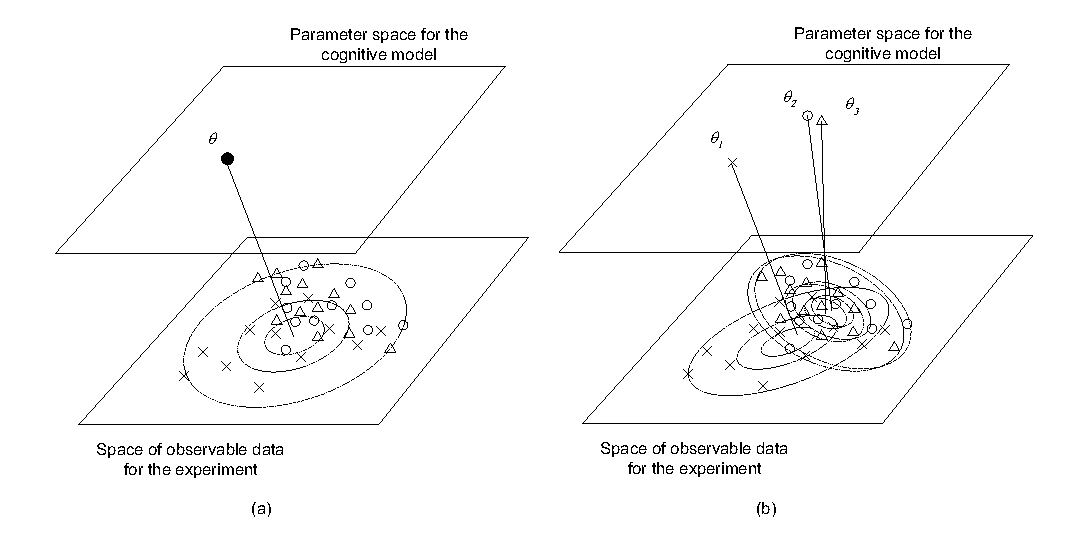
\epsfig{file=conventionalview.eps,width=15cm}
        \caption{\bfc Standard modeling approaches for data from many subjects, involving the aggregation of data (panel a), and the modeling of each individual independently (panel b).
        The data are plotted in the lower data space, with different symbols for each
        participant. The upper parameter space shows the parameter distributions inferred under each modeling approach.\efc}
        \label{conventionalview}
        \end{center}
\end{figure}

Notwithstanding the ongoing debate about the  relative merits of fitting
aggregated versus individual data (e.g., Maddox \& Estes, 2005),
the previous discussion suggests that \emph{both} viewpoints are unsatisfying.
To provide a visual illustration of this point, consider the hypothetical data
shown in Figure~\ref{conventionalview}.
The figure depicts the outcome of  a simple experiment in which we collect
noisy data from three participants. The three participants' data are indicated with crosses,
 circles, and triangles. The crosses form a roughly elliptical
shape from the lower left to the upper right of the data space, whereas the circles
and triangles form ellipses that slant from the upper left to the lower right. On the
left hand side (panel a), we aggregate across participants, and estimate a single
parameter value $\theta$ that produces a distribution that is roughly circular,
indicated by the contour plot. The aggregate looks nothing like the individuals. On the right hand side (panel b),
we estimate a parameter value independently for each participant. The  inferred parameter values $\theta_1$, $\theta_2$ and $\theta_3$ and their associated contour plots now do capture the basic aspects of everyone's performance. However, this accuracy has come at the cost of losing sight of the similarity between two of the
participants. Using the individual
fitting approach, this relationship $\theta_2 \approx \theta_3$ is not represented. Even if we observed a
large number of people with very similar parameter values, we could make no formal inference about the relationship between them. Ultimately, neither the aggregate nor the individual view captures the pattern of similarities and differences apparent in the data. Aggregated models can learn similarities and individual models
can learn differences, but modeling individual variation in cognition requires being able to learn both simultaneously.

\begin{figure}[t]
        \begin{center}
        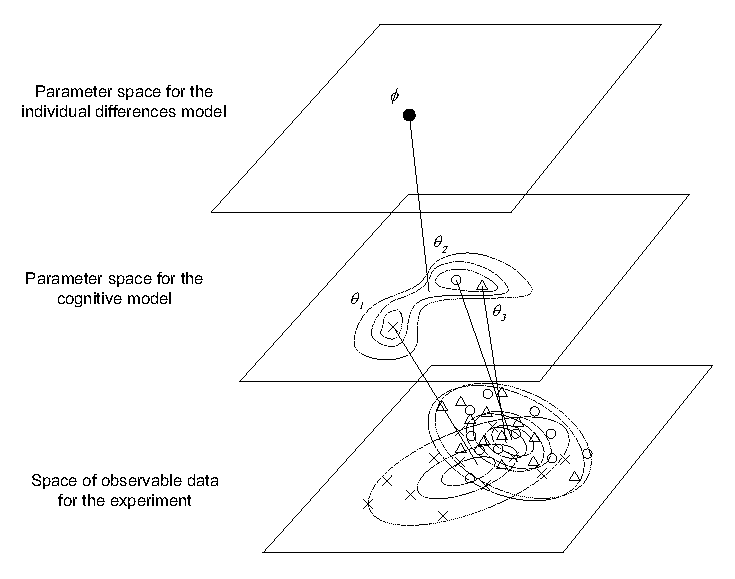
\epsfig{file=modelview.eps,width=11cm}
        \caption{\bfc The model-based view of individual differences. The data are plotted in the lower data space, with different symbols for each
        participant. The middle parameter space shows the parameter values inferred for each participant based on their data {\it and} an individual differences model that describes how these parameters can vary between people. The upper parameter space shows the inferred parameter values for this individual differences model. \efc}
        \label{modelview}
        \end{center}
\end{figure}

Because of these difficulties, a number of authors have considered
more sophisticated ways of expressing individual differences within models of cognitive processes (e.g., Lee \& Webb, in press; Peruggia, Van Zandt \& Chen,
2002; Rouder, Sun, Speckman, Lu \& Zhou, 2003; Steyvers, Tenenbaum,
Wagenmakers \& Blum, 2003; Webb \& Lee, 2004). The central innovation
is to provide an explicit model for the kinds of individual differences that might
appear in the data, in much the same way as established methods in psychometric models like Item Response Theory
(e.g., Lord, 1980; Hoskens \& de Boeck, 2001; Junker \& Sijtsma, 2001). The general approach, illustrated schematically in Figure~\ref{modelview}, is to supplement the cognitive model  that describes variation within a single participant's data with an individual differences model that describes
\emph{how} cognitive parameters can vary across people. Using sufficiently flexible individual differences models, it is possible to learn both the similarities
and differences between people.

Model-based approaches to individual differences vary in terms of the class
of distributions that are allowed to describe variation in parameter values,
reflecting different assumptions about which aspects of individual differences
are the most important to capture. In this paper we introduce a new model-based
framework for understanding individual differences. Informed by
recent insights in statistics and machine learning (e.g., Escobar \& West,
1995; Neal, 2000), our \emph{infinite groups model} makes it possible to
divide subjects who behave similarly into groups, without assuming an
upper bound on the number of groups. This
model is sufficiently flexible to capture the heterogeneous structure produced
by different subjects pursuing different strategies, allows the number of
groups in the observed sample to grow naturally as more data appear,
and avoids the complex computations that are often required when one
chooses an individual differences model by standard model selection methods.
We illustrate the infinite groups model by considering
simple multinomial models that predict the frequencies of responses across
a set of categories. However, the idea generalizes to more general classes of
probabilistic models.

The structure of the paper is as follows: We begin with an overview of
existing frameworks for modeling individual differences, and their
interpretations as Bayesian hierarchical models. We then introduce
the infinite groups approach as a principled way to address some of the
problems associated with these frameworks, including model selection
problems. Next, we provide a brief tutorial on the Dirichlet process,
which forms the basis of our approach, and discuss how model selection
proceeds when working with the infinite groups framework.
We then derive the infinite groups model for discrete
data and present illustrative simulation studies. Finally, we present
three applications that analyze the individual differences
in categorization performance, choice of publication
outlets, and web browsing behavior.

\section{Hierarchical Bayesian Models for Individual Differences}

Two dominant model-based approaches have emerged in the literature on
individual differences. In a \emph{stochastic parameters model}
(e.g., Peruggia et al., 2002; Rouder et al., 2003), every participant
is assumed to have a unique parameter value $\theta$ that is
sampled from a parametric distribution, as illustrated in
Figure~\ref{existing}\panel{a}. The intuition behind the approach is that,
while every person is unique, the variation between people is not arbitrary,
and can be described by a distribution over the parameters. These
distributions are generally smooth and unimodal, reflecting a general
tendency at the mode, and a noise model describing the
variations that exist across individuals' parameters.
In contrast, the idea that underlies the \emph{groups model}
is that there exist a number of distinct types of
qualitatively different performance. Accordingly, this approach assumes that people fall
into one of a number of fundamentally
distinct groups. Within a group, people are assumed to behave in
 the same way, but the groups themselves can vary in all kinds of ways.
 Under this approach to individual differences modeling
(e.g., Lee \& Webb, in press; Steyvers et al., 2003; Webb \& Lee, 2004),
the goal is to partition subjects into a number of groups and associate each
group with a parameterization $\theta$, as illustrated in Figure~\ref{existing}\panel{b}.


In order to understand the assumptions that underlie these two
frameworks, it is helpful to view them as {\em hierarchical
Bayesian models} (e.g., Lindley \& Smith, 1972). Suppose we have
data from an experiment that involves $n$ participants. If the $i$th
individual participant provides $m_i$ observations, we can denote
these observations by the vector $\vctr{x}_{i}=(x_{i1}, \ldots, x_{i \,m_i})$.
By specifying a cognitive model, we assume that these
data can be described as {\it i.i.d.} samples from the distribution
$x_{ij} \sim F(\cdot \condon \theta_i)$.  Additionally, by specifying an individual differences model, we assume
that there is a distribution $\theta_i \sim G(\cdot \condon \vctr{\phi})$
that we can use to describe the parameter values $\vctr{\theta}=
(\theta_1, \ldots, \theta_n)$ for each of the participants. Since we
now have two distinct levels at which we wish to construct models,
we can write a model of this form as the two-level hierarchical model,
\begin{equation}
        \begin{array}{rcl}
        x_{ij} \condon \theta_i & \sim & F(\cdot \condon \theta_i)\\
        \theta_i \condon \vctr{\phi} & \sim & G(\cdot \condon \vctr{\phi}).
        \end{array}
        \label{hmod}
\end{equation}
\noindent In this expression $\vctr{\phi}$ denotes the parameters used
to describe the individual differences model $G(\cdot \condon \vctr{\phi})$.
Letting $\vctr{x}=(\vctr{x}_1,
\ldots, \vctr{x}_n)$ refer to the complete data set, we can write the
likelihood function for this hierarchical Bayesian model as,
\begin{eqnarray}
        p(\vctr{x} \condon \vctr{\phi})  &=&
        \prod_i p(\vctr{x}_i \condon \vctr{\phi})  \nonumber \\
        &=& \prod_i \int \left( \prod_j  F(x_{ij} \condon \theta_i) \right)
        G(\theta_i \condon \vctr{\phi}) \, \mathrm{d}\theta_i.
\end{eqnarray}
To apply Bayesian inference to this model, we also need to define a prior
on $\vctr{\phi}$. We will assume that $\vctr{\phi} \sim \pi(\cdot)$ for
some appropriate distribution $\pi(\cdot)$. Statistical inference in this
model is achieved by finding $p(\vctr{\theta}, \vctr{\phi} \condon \vctr{x})$,
the joint posterior distribution over parameter values and individual difference
models. However, we are often only interested in some aspects of this joint
posterior, so only some parts are reported. Two cases of particular interest are,
\begin{enumerate}
\item {\it Posterior over parameters for the cognitive model}. One role of $G(\cdot \condon \vctr{\phi})$
is to induce dependencies between the parameters $\theta_i$. In some contexts
this is all that the researcher requires, so it is natural in these situations to
consider the marginal distribution $p(\vctr{\theta} \condon \vctr{x})$. The idea
in this case is that we would use the dependencies induced via our individual
differences model to produce better parameter estimates.
\item {\it Posterior over the parameters for the individual differences model}. A second role for
$G(\cdot \condon \vctr{\phi})$ is to provide a theoretical account of the
variation across the parameters $\theta_i$. In those contexts, the researcher
may wish to report the marginal distribution $p(\vctr{\phi} \condon \vctr{x})$.
The idea in this case is to learn the structure of individual variation from the data.
\end{enumerate}

In this paper we are interested more in the second case than the first, and
it is necessary to distinguish between the two. This is particularly important
since stochastic parameter models are generally motivated by the first
case, while group models are often applied
in the second. This difference in focus is reflected in the fact that, while
 both stochastic parameter models and group models can be viewed
as hierarchical models, they differ in the form of the distribution $G(\cdot
\condon \vctr{\phi})$ that describes individual variation. In the stochastic
parameters model, $G(\cdot \condon \vctr{\phi})$ is usually a tractable
distribution such as a Gaussian, with $\vctr{\phi}$ corresponding to
the parameters of that distribution, as in Figure~\ref{existing}\panel{a}.
In contrast, if we have a model with $k$ groups, the individual differences
model $G(\cdot \condon \vctr{\phi})$ is a weighted collection of
$k$ point masses, as depicted in Figure~\ref{existing}\panel{b}. That is,
\begin{equation}\label{finitegroups}
        G(\cdot \condon \vctr{w},\vctr{\theta}) = \sum_{z=1}^k w_z \,
        \delta(\cdot \condon \theta_z),
\end{equation}
where $\delta(\cdot \condon \theta_z)$ denotes a point mass distribution
located at $\theta_z$ and where $\sum_{z=1}^k w_z =1$. In the groups
model, $\vctr{\phi} = (\vctr{w},\vctr{\theta})$. It is important to notice
that in this expression, $\vctr{\theta}$ refers to the locations of the $k$
spikes that make up the distribution $G(\cdot \condon \vctr{w},\vctr{\theta})$
and are thus parameters of the individual differences model. The parameter
values for the individual subjects are then sampled from this distribution,
and are all equal to one of these $k$ values. Notationally, we will distinguish
between these two uses through the subscripts: $\theta_i$ will denote the
parameters for the $i$th participant, while $\theta_z$ will denote parameter for
group $z$. If the subscript is ambiguous, we will make it clear in each context.

The hierarchical Bayesian model perspective reveals some of the strengths and
weaknesses of the two approaches. Assuming that individual parameters
$\theta_i$ follow a simple parametric distribution, as in the stochastic
parameters model, simplifies the problem of learning an individual differences
model from data, but places strong constraints on the kind of variation that
can manifest across subjects.  A particularly severe problem arises when we
specify a unimodal distribution to capture individual differences that are
inherently multimodal, perhaps arising from different interpretations of
a task. In this case the model cannot capture the most
important aspect of the variation between people. Unimodal distributions naturally suggest an interpretation
in terms of variation away from a single prototypical parameter value
at the mode, which is misleading in many situations. To return to
the unlucky numbers experiment, we might end up estimating a
distribution with a mean of about 17, and a large enough variance to
capture the performance of the individual subjects. While this account
may provide reasonable estimates of the individual parameters (case 1),
it is unsatisfactory as an explanation of these parameters (case 2).
We would prefer to recognize that
the data here have three distinct modes, located at 4, 13, and 87.

Unlike the stochastic parameters approach, the parameter distributions
allowed by group models can naturally account for multimodality in
individual differences. By postulating two groups, for instance, we arrive
at a bimodal distribution. While this is desirable, given our goal of learning
group structure from data, it introduces the problem of how many groups
we should include in our individual differences model. In finite group models,
this is viewed as a model selection problem. The fixed number of groups $k$ is taken
to define a family of individual differences distributions $\mathcal{M}_k$,
and we are required to determine which of these families is best for our data.
As a result, model selection issues are central to the application of group
models to psychological data, and often make statistical inference very
difficult computationally. In this paper we explore an {\it infinite groups models}, which retains
the flexibility of the finite groups model but allows straightforward inference.
Questions of model selection will still arise, but in a different and more theoretically
satisfying fashion.

\begin{figure}[t]
        \begin{center}
        \begin{tabular}{ccc}
        \hspace*{-5mm}
        \protect\raisebox{0mm}{\epsfig{file=unimodal.eps,width=5cm}}
        &\hspace*{-5mm}
        \protect\raisebox{0mm}{\epsfig{file=partitioning.eps,width=5cm}}
        & \hspace*{-3mm}
        \protect\raisebox{3mm}{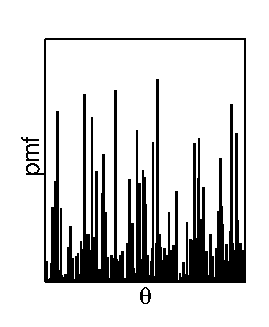
\epsfig{file=infgpspic.eps,width=4.7cm}} \\
        (a) &(b) &(c)\end{tabular}
        \caption{\bfc Parameter distributions \fcs
        associated with stochastic parameters approach \fcs to individual
        differences (panel a), the \fcs original groups approach (panel b), and
        the infinite groups approach (panel c). The continuous measure shown
        in panel a is a probability density function (pdf) while the discrete
        measures in panels b and c are probability mass functions (pmf).\efc}
        \label{existing}
        \end{center}
\end{figure}

\section{The Infinite Groups Model}

Although the infinite groups model has implications for the model selection
problem, it is motivated by a more psychological concern with finite
group models. The statistical model described in Equation~\ref{finitegroups}
assumes that $k$ is a fixed value, independent of sample size. Such a
model requires, rather implausibly, that future subjects will belong to one
of the same set of $k$ groups that were observed previously. No provision
is made in this model for the idea that, should more data be observed, more
groups could be observed. In contrast, we start with the assumption that
there are an {\it infinite} number of latent groups, only some number of
which are observed in any finite sample. The consequence is that $k$ is
now variable, and can grow with the data.

To build the infinite groups model, we adopt a distribution on individual
parameters $\vctr{\theta}$ that is more flexible than the parametric
distribution assumed by the stochastic parameters model, but still allows
efficient inference. We assume that subjects are drawn from an infinite
number of groups, taking $G(\cdot \condon \vctr{\phi})$ to be a
weighted combination of an infinite number of point masses, as in
Figure~\ref{existing}\panel{c}. That is, the individual
differences model is assumed to be of the form,
\begin{equation}
        \label{infpointmasses}
        G(\cdot \condon \vctr{w},\vctr{\theta}) =
        \sum_{z=1}^{\infty} w_z \, \delta(\cdot \condon \theta_z).
\end{equation}
\noindent Once again, $\delta(\cdot \condon \theta_z)$ denotes a
point mass distribution located at $\theta_z$, and since the $w_z$
values denote mixture weights, they must sum to 1. While we assume
that the number of groups is unbounded, any finite set of subjects will
contain representatives from a finite subset of these groups. This model
is psychologically plausible: People can vary in any number of ways,
only some of which will be observed in a finite sample. With infinitely
many groups, there is always the possibility that a new subject can
display behavior that has never been seen before.

\subsection{Finite-Dimensional Priors}

In order to apply Bayesian inference in the hierarchical model defined by
Equations~\ref{hmod} and~\ref{infpointmasses}, we need to define a prior
$\pi(\cdot)$ over the possible individual differences models $G(\cdot)$.
A specific individual differences model is defined by the the countably infinite
number of elements of $\vctr{w}$ and $\vctr{\theta}$ in Equation
\ref{infpointmasses}, where $w_z$ denotes the probability that
$G(\cdot)$ assigns to the $z$th point mass, and $\theta_z$ denotes the
location of that point mass. In other words, we need a prior over the infinite
dimensional space $\mathcal{W} \times\Theta$ that covers the possible values
for the parameter vectors $\vctr{w} \in \mathcal{W}$ and $\vctr{\theta} \in
\Theta $. To see how we might place a sensible prior on this infinite dimensional
space, it is helpful to consider how we might proceed in the finite case when
$G(\cdot)$ consists of only $k$ point masses, and then take the limit as
$k \rightarrow \infty$. This approach is a standard way of eliciting
infinite-dimensional priors  (e.g., Neal, 2000; Rasmussen, 2000; Green
\& Richardson, 2001; Griffiths \& Ghahramani, 2005). Note that this procedure
does not explicitly derive the prior distribution itself. Rather, it provides a
principled motivation for a particular choice of prior.

In a finite groups model with $k$ groups (i.e., Equation~\ref{finitegroups}),
 a standard prior is
\begin{equation}
        \begin{array}{rcl}
        \theta_z & \sim & G_0(\cdot) \\
        \vctr{w} \condon \alpha, k & \sim &
        \mbox{Dirichlet}(\cdot \condon \vctr{\zeta}).
        \end{array}
        \label{finiteprior}
\end{equation}
\noindent In this prior, each of the $k$ location parameters $\theta_z$ is
sampled independently from the \emph{base distribution} $G_0(\cdot)$.
This base distribution provides a prior over the kinds of parameter values
that are likely to capture human performance in a particular task. Choosing
the base distribution is no different to setting a prior in any other Bayesian
context, and so this prior should be chosen in the usual way. That said,
there are differing views as to what ought to be the `usual way'
(e.g.,  de Finetti, 1974; DeGroot; 1970; Kass \& Wasserman, 1996;
Jaynes, 2003), but it is outside the scope of this paper to discuss this
debate between subjective and objective views of Bayesian inference.
Whatever approach is adopted, the base distribution $G_0(\cdot)$
is not affected when we make the transition from finite models
to infinite models.

For our purposes, the relevant part of this prior is the distribution over the
weights. Placing a prior over the weights is made difficult by the constraint
that they need to sum to 1. Typically, in the finite case, we would use a
$k$-dimensional Dirichlet distribution as a prior over these weights. The
general form for a $k$-dimensional Dirichlet with parameters
$\vctr{\zeta}=(\zeta_1,\ldots,\zeta_k)$ is given by,
\begin{equation}
        p(\vctr{w}\condon \vctr{\zeta}) = \frac{1}{\dnorm(\vctr{\zeta})}
        \left( \prod_{z=1}^{k} w_z^{\zeta_z-1}\right) I(\vctr{w}),
\end{equation}
where $I(\vctr{w})=1$ if the weights $\vctr{w}$ sum to 1, and
$I(\vctr{w})=0$ otherwise. The Dirichlet distribution is a higher-dimensional
version of the Beta distribution, with the Beta distribution corresponding to
the case where $k=2$.
The normalizing function $\dnorm(\vctr{\zeta})$
for the Dirichlet distribution is given by
\begin{eqnarray}
        \label{dirnorm}
        \dnorm(\vctr{\zeta}) &=& \int  \left( \prod_{z=1}^{k} w_z^{\zeta_z-1} \right)
        I(\vctr{w}) \, \mathrm{d}\vctr{w} \nonumber \\
        &=&\frac{\prod_{z=1}^k \Gamma \left(\zeta_z \right)}
        {\Gamma \left(\sum_{z=1}^k \zeta_z\right)}.
\end{eqnarray}
In this expression $\Gamma(y)=\int_0^\infty u^{y-1}e^{-u} \, \mathrm{d}u$ is the
standard Gamma function, which generalizes the factorial function: If $y$ is
a non-negative integer, then $\Gamma(y+1)=y!$ When the Dirichlet distribution is used
as a prior in a finite groups model, it is typical to use a symmetric Dirichlet distribution
in which all parameters are equal. The reason for using a symmetric
distribution stems from the prior being insensitive to the ordering of the location
parameters $\vctr{\theta}$. Since the location parameters are
independent of one another, their order (i.e., the value of the index $z$) is irrelevant.
This exchangeability requires that the prior over $\vctr{w}$ be set
so that the index is also irrelevant, which is achieved by setting a
symmetric prior.

For the purposes of deriving a prior over infinite groups, we will assume that all
parameter values $\zeta_z$ are set to $\alpha/k$.
The choice of $\alpha/k$ as the parameter value follows from
recognizing that the sum of the parameters of a Dirichlet distribution can be
 interpreted as indicating how heavily to weight the prior.  To understand this property
of the Dirichlet parameters it may help to
consider an example using an idealized bent coin. Suppose that data
are produced by $n$ independent flips of a bent coin. We might propose a simple
model, in which these are {\it i.i.d.} Bernoulli trials with an unknown probability
$p$ of obtaining a head. The prior we set over this unknown $p$ could be Dirichlet
with only $k=2$ possible outcomes, corresponding to a Beta distribution. Since we do not
know which way the coin is bent, the distribution over $p$ should be symmetric.
We will set the parameters to $\alpha/2$. If we then observe $h$ heads and
$t=n-h$ tails in our data, our posterior distribution is still a Beta, since the Beta family
is conjugate\footnote{A family of prior distributions is conjugate to
a particular likelihood function if the posterior distribution belongs to the same family as
the prior (e.g., Bernardo \& Smith, 2000, pp.~265--285).}
to the Binomial likelihood. The parameters of the posterior Beta are
$h+\alpha/2$ and $t+\alpha/2$.
As a result, the expected posterior value of $p$ is
$\bar{p} = (h + \alpha/2)/(n+\alpha)$. From the denominator, it is evident
that $\alpha$ is commensurate with $n$, in terms of its influence on this estimate.
This property generalizes to larger $k$. Our goal here is to specify a prior over
an infinite-dimensional outcome space $\mathcal{W}$ that embodies only a limited
amount of information, so it is helpful to choose the prior in a way that keeps the
amount of information independent of the dimensionality $k$.
The $\alpha/k$ prior achieves this by ensuring that the sum of the parameter
vector is always $\alpha$. For more details on the $\alpha/k$ prior, see Neal (2000)
and Ishwaran and Zarepour (2002).

To find the limiting prior as $k \rightarrow \infty$, it is helpful to to
rewrite the finite-dimensional model in a
way that lets us integrate out $\vctr{w}$. To do this, we introduce the group
membership variable $g_i$,  indicating the group to which the $i$th observation
belongs.  Since $w_z$ gives the probability that the $i$th observation belongs to the
$z$th group, we can say that $p(g_i=z \condon \vctr{w})=w_z$.  With this
membership variable introduced, the finite-dimensional model with this prior
becomes,
\begin{equation}
        \begin{array}{rcl}
        x_{ij} \condon \vctr{\theta}, g_i=z & \sim & F(\cdot \condon \theta_z) \\
        g_i \condon \vctr{w} & \sim & \mbox{Multinomial}(\cdot \condon\vctr{w}) \\
        \vctr{w} \condon \alpha, k & \sim & \mbox{Dirichlet}(\cdot \condon
        \frac{\alpha}{k}) \\
        \theta_z \condon G_0 & \sim & G_0(\cdot),
        \end{array}
        \label{finiteprior2}
\end{equation}
where the multinomial is of sample size one. Since the group assignment variables $g_i$ are
conditionally independent given the weights $\vctr{w}$, when we integrate out the
weights we induce a conditional dependence between the group assignments. If we have
observed the first $i-1$ group assignments $\vctr{g}_{-i} = (g_1, \ldots, g_{i-1})$, we want
the conditional probability $p(g_i=z \condon \vctr{g}_{-i}, \alpha, k)$ that is obtained by
integrating out $\vctr{w}$. This distribution is given by,
\[
        p(g_i=z \condon \vctr{g}_{-i}, \alpha, k) = \int p(g_i=z \condon \vctr{w})
        p(\vctr{w} \condon \vctr{g}_{-i}, \alpha, k) \, \mathrm{d}\vctr{w}.
\]
We have already seen that  $p(g_i=z \condon \vctr{w})=w_z$. By applying Bayes'
theorem we observe that the second term is the posterior probability,
\[
        p(\vctr{w} \condon \vctr{g}_{-i}, \alpha, k) \propto p(\vctr{g}_{-i } \condon \vctr{w})
        p(\vctr{w} \condon \alpha, k).
\]
Since the first term is a multinomial probability and the second term is Dirichlet,
conjugacy implies that the posterior is also Dirichlet. If we let $s_z$ denote the number of
previous observations that were assigned to group $z$, we can use the size vector
$\vctr{s}=(s_1, \ldots, s_k)$ to indicate how many observations fall in each group.
The posterior probability $p(\vctr{w} \condon \vctr{g}_{-i}, \alpha, k)$ is a
non-symmetric Dirichlet with the parameter vector $\vctr{s} + \alpha/k$.
We can now solve the integral.
\begin{eqnarray}
        p({g}_i=z \condon \vctr{g}_{-i}, \alpha, k)&=&
        \frac{1}{\dnorm(\vctr{s}+\frac{\alpha}{k})}
        \int w_z \left(  \prod_u w_u^{s_u +\frac{\alpha}{k} -1} \right)
        I(\vctr{w}) \, \mathrm{d}\vctr{w}  \nonumber \\
        &=& \frac{\dnorm \left(\vctr{s}+\frac{\alpha}{k}+ \mathbf{1}^{(z)}\right) }
        {\dnorm \left(\vctr{s}+\frac{\alpha}{k}\right)} \nonumber \\
        &=& \frac{s_{z} + \frac{\alpha}{k}}{i-1+\alpha}.
\end{eqnarray}
In this expression, $\mathbf{1}^{(z)}$ is a $k$-length vector of zeros with a 1
in position $z$. The last line follows from Equation~\ref{dirnorm} and the fact
that $\Gamma(y+1)= y \Gamma(y)$.

\subsection{Extension to Infinite-Dimensional Priors}

The finite-dimensional prior can now be extended to the infinite case by letting
$k\rightarrow \infty$ (see Neal, 2000; Ishwaran \& Zarepour, 2002).
Consider first the probability that the $i$th observation
falls in a group $z$ that already contains at least one member (i.e. $s_z>0$). In
this case, the limiting probability is
\begin{eqnarray}
        p(g_i=z \condon \vctr{g}_{-i}, \alpha) &=& \lim_{k \rightarrow \infty}
        \left( \frac{s_{z} + \frac{\alpha}{k}}{i-1+\alpha} \right) \nonumber \\
        &=& \frac{s_{z}}{i-1+\alpha}. \label{crpexpand1}
\end{eqnarray}
We now consider the probability that the $i$th observation falls in one of the
infinitely many groups that as yet contain no observations. If there are $k_{-i}$
groups observed among the first $i-1$ observations, and letting $\mathcal{Q}$
denote the  set of $k-k_{-i}$ currently empty groups, then the probability that
the $i$th observation belongs to one of them is,
\begin{eqnarray}
        p(g_i \in \mathcal{Q}  \condon \vctr{g}_{-i}, \alpha)
        &=& \lim_{k \rightarrow \infty} \left(\sum_{u \in \mathcal{Q}} \frac{s_{u}
        + \frac{\alpha}{k}}{i-1+\alpha} \right) \nonumber \\
        &=& \frac{ \alpha}{i-1+\alpha} \, \lim_{k \rightarrow \infty}
        \left(\frac{k-k_{-i}}{k} \right) \nonumber \\
        &=& \frac{\alpha}{i-1+\alpha}. \label{crpexpand2}
\end{eqnarray}
Notice that $\alpha$ remains commensurate with sample size in the limiting
prior (in the derivation above the sample size is $i-1$) and so can be
interpreted as a measure of prior information. In the bent coin example,
$\alpha$ acted to drag the estimator toward the prior, thereby shaping
predictions about future data. In the infinite groups model, large
$\alpha$ increases the probability that future data will be drawn from a
previously unobserved group. Since new groups have parameter values drawn
from the prior $G_0(\cdot)$, larger $\alpha$ increases the influence of
the prior. Moreover, since large $\alpha$ values tend to introduce more
groups, it can be thought of as a \emph{dispersion} parameter.

The group assignments $g_i$ define a partition of the subjects, with each
subject being assigned to a single group. The distribution over partitions
induced by taking the limit of a Dirichlet-multinomial model, as we did in
Equations 10 and 11, is the same as that induced by a stochastic process
called the {\it Chinese Restaurant Process} (CRP: e.g., Aldous, 1995;
Pitman, 1996) with dispersion $\alpha$.  The CRP gets its name from a
metaphor based on Chinese restaurants in San Francisco that seem to have
limitless seating capacity. In this metaphor, every possible group
corresponds to a table in an infinitely large Chinese restaurant. Each
observation corresponds to a customer entering the restaurant and sitting
at a table. People are assumed to prefer sitting at popular tables (with
probability proportional to the number of people already sitting at the
table), but it is always possible for them to choose a new table (with
probability proportional to $\alpha$). This gives exactly the conditional
distribution over group assignments obtained in Equations~\ref{crpexpand1}
and~\ref{crpexpand2}, with the joint distribution over group assignments
written $\vctr{g} \condon \alpha \sim \mbox{{\it CRP}}\,(\cdot \condon
\alpha)$. The resulting model becomes
\begin{equation}
        \label{igm_crp}
        \begin{array}{rcl}
        x_{ij} \condon \theta_z, g_i=z & \sim & F(\cdot \condon \theta_z)\\
        \vctr{g} \condon \alpha &\sim& \mbox{{\it CRP}}\,(\cdot \condon \alpha) \\
        \theta_z \condon G_0 & \sim & G_0(\cdot).
        \end{array}
\end{equation}
To complete the motivation of our prior, it is helpful to find the prior
distribution over parameter values $\theta_i$, by integrating out the group
assignment variables $g_u$. Since these are just indicator variables, this is
straightforward:
\begin{equation}
        \theta_{i} \condon \vctr{\theta}_{-i},  \alpha, G_0 \sim
        \frac{\alpha}{i-1+\alpha} G_0(\cdot) + \sum_{z=1}^{k_{-i}}
        \frac{s_z}{i-1+\alpha}  \delta(\cdot \condon {\theta_z}).
        \label{pus}
\end{equation}
To avoid confusion, it is important to recognize that $\theta_z$ denotes the
parameter value associated with all the members of group $z$, whereas
$\vctr{\theta}_{-i}=(\theta_1, \ldots, \theta_{i-1})$ denotes parameters assigned
to particular observations, as does $\theta_i$. The conditional probability
described in Equation~\ref{pus} is a mixture between the empirical
distribution of the $i-1$ previously observed parameters and the base
distribution $G_0(\cdot)$.

A sequence of parameter values sampled from Equation~\ref{pus} is sometimes
said to be sampled from a {\it P\'{o}lya urn} (PU: e.g., Blackwell \& MacQueen,
1973) parameterized by $G_0(\cdot)$ and $\alpha$. In a P\'{o}lya urn
scheme, we imagine an urn full of $\alpha$ colored balls, such that the proportion of
balls with color $\theta$ is equal to $G_0(\theta)$. We sample $\theta_1$
 by drawing a ball at random from the urn and recording its color. We then return the ball to
 the urn and drop in another ball of the same color, effectively ``updating'' the urn.
Using this P\'{o}lya urn formulation to express the induced prior on $\theta$, our
model may be written,
\begin{equation}
        \label{igm_pus}
        \begin{array}{rcl}
        x_{ij} \condon \theta_i & \sim & F(\cdot \condon \theta_i)\\
        \theta_1, \ldots, \theta_\infty \condon G_0, \alpha &\sim&
        \mbox{{\it PU}}\,(\cdot \condon G_0, \alpha).
        \end{array}
\end{equation}
This description now allows
us to select an appropriate infinite-dimensional prior: We want to choose
a prior over the individual differences distribution $G(\cdot)$, subject to the
constraint that the marginal prior over the set of individual parameters
$\theta_1, \ldots, \theta_\infty$ is a P\'{o}lya urn scheme. As noted by
Blackwell and MacQueen (1973), one prior that meets
this requirement is the \emph{Dirichlet process} (DP: Ferguson, 1973).

\begin{figure}[t]
       \begin{center}
        \begin{tabular}{ccccc}
        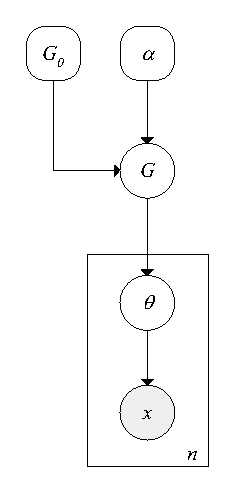
\epsfig{file=dp_classic2.eps,width=2.9cm}& \hspace*{-3mm}  &
        \protect\raisebox{0mm}{\mbox{\epsfig{file=stickdp.eps,width=3.6cm}}} &
        \hspace*{-5mm} &
        \protect\raisebox{1mm}{\mbox{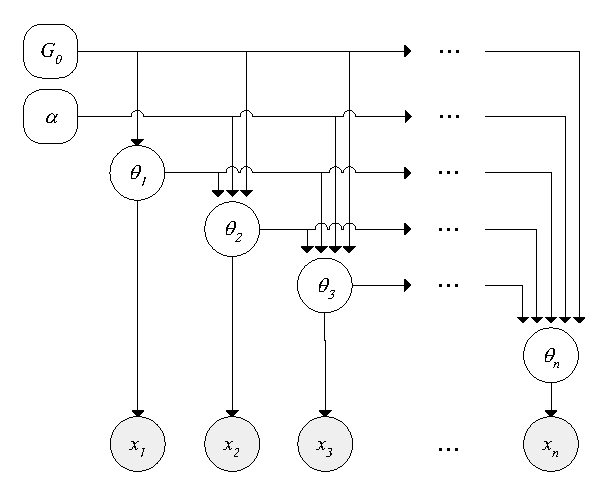
\epsfig{file=dp_crp2.eps,width=8cm}}}
        \\ (a) & & (b) & & (c)
        \end{tabular}
        \caption{Three graphical representations of a model employing a Dirichlet
        process prior. Each panel depicts the same model, but shown from a different
        perspective. Panel a depicts the standard view (Equation~\ref{igm}),
        panel b shows the Sethuraman construction (Equation~\ref{infiniteprior})
        and panel c displays the construction via the P\'{o}lya urn scheme
        (Equation~\ref{igm_pus}). \efc}
        \label{dpmodels}
        \end{center}
\end{figure}

The Dirichlet process is widely used in nonparametric Bayesian statistics as
a method for placing priors on infinite mixture models (e.g., Lo, 1984;
Escobar \& West, 1995;  Rasmussen, 2000; Neal, 1996, 2000;
Blei, Griffiths, Jordan \& Tenenbaum, 2004), and has
sometimes been applied in psychometrics as a  generic prior over probability
distributions in Bayesian Item Response Theory models (e.g., Duncan, 2004;
Qin, 1998). This connection between the Dirichlet process and the P\'{o}lya urn
scheme suggests that our prior on the individual differences distribution
should be a Dirichlet process. Having elicited a principled prior, we may now
formally specify the infinite groups model in the following way:
\begin{equation}
        \label{igm}
        \begin{array}{rcl}
        x_{ij} \condon \theta_i & \sim & F(\cdot \condon \theta_i)\\
        \theta_i \condon G & \sim & G(\cdot) \\
        G \condon G_0, \alpha &\sim& DP(\cdot \condon G_0, \alpha).
        \end{array}
\end{equation}
This model is illustrated graphically in Figure~\ref{dpmodels}\panel{a}. Parameters
arise from an unknown distribution $G(\cdot)$, and our uncertainty about this
distribution is reflected through the Dirichlet process prior.
Grey circles denote
observed variables, white circles denote latent variables, and the rounded squares
denote parameters whose values are assumed to be known. Plates indicate a
set of independent replications of the processes inside them (Buntine, 1994).
For comparison, the P\'{o}lya urn formulation in Equation~\ref{igm_pus} is
shown in panel~c.

\section{The Dirichlet Process}

In nonparametric problems, the goal is to learn from data without making any
strong assumptions about the class of parametric distributions (e.g., Gaussian)
that might describe the data. The rationale for the approach is that the generative
process for a particular data set is unlikely to belong to any finite-dimensional parametric
family, so it would be preferable to avoid making this false assumption at the outset.
From a Bayesian perspective, nonparametric assumptions require us to place a prior
distribution that has broad support across the space of probability distributions.
However, Bayesian nonparametrics are not widely known in psychology (but see
Karabatsos, in press), so a brief discussion may be helpful.

The Dirichlet process, now a standard prior in Bayesian nonparametrics, was
constructed by Freedman (1963) during a discussion of {\it tail-free processes},
and the associated statistical theory was developed by Ferguson (1973, 1974).
The Dirichlet process represents a partial solution to the problem of Bayesian
nonparametric inference, in the sense that it does have broad support, but the
sampled distributions are discrete with probability 1 (e.g., Ferguson, 1973;
Blackwell, 1973; Sethuraman, 1994; Ghosh \& Ramamoorthi, 2003, pp.~102-103).
As a result it is often used as a prior over discrete distributions\footnote{One
reason for the popularity of the Dirichlet process is tractability, since
the Dirichlet process is conjugate to {\it i.i.d.}\ sampling
(Ferguson, 1973). If the prior over $G(\cdot)$ is a Dirichlet process with
parameters $\alpha$ and $G_0(\cdot)$, and we observe {\it i.i.d.}\ data with
empirical distribution $G_n(\cdot)=\frac{1}{n} \sum_{i=1}^n
\delta(\cdot \condon \theta_i)$, then the posterior distribution over $G(\cdot)$ is a
Dirichlet process with dispersion $\alpha + n$ and base distribution
$\frac{\alpha}{\alpha+n}G_0(\cdot) + \frac{n}{\alpha+n} G_n(\cdot)$.
However, it is important to note that since
the Dirichlet process concentrates on discrete distributions, it can be unsuitable
as a prior over densities. For instance, Diaconis and Freedman (1986) provide an
example of pathological behavior when the Dirichlet process is used in this way.}
and it is in this capacity that we have used the Dirichlet process in this paper.
Since we require an infinite number of variables (the countably infinite elements
of $\vctr{w}$ and $\vctr{\theta}$) to describe a sample from the Dirichlet
process, it is often referred to as an {\it infinite-dimensional model}.

\begin{figure}[t]
        \begin{center}
        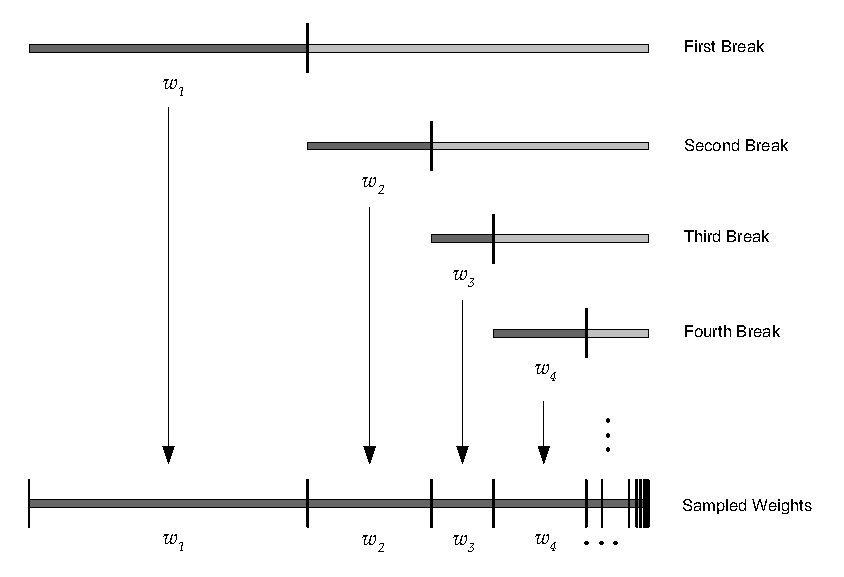
\epsfig{file=stickprocess.eps,width=13.7cm}
        \caption{A graphical depiction of the stick-breaking process, showing
        successive breaks of a stick with starting length one, and how the lengths
        of the pieces correspond to sampled weights.\efc}
        \label{stickbreaking}
        \end{center}
\end{figure}

\subsection{Stick-Breaking Priors}

The simplest description of the Dirichlet process is as an
example of a {\it stick-breaking prior} (e.g., Ishwaran \& James, 2001; Ishwaran
\& Zarepour, 2002). This construction was first discussed by McCloskey (1965),
and formalized by Sethuraman (1994). In this formulation,  we start by noting
that discrete distributions can be written
\[
        G(\cdot)=\sum_{z=1}^{\infty} w_z \, \delta(\cdot \condon \theta_z),
\]
as per Equation~\ref{infpointmasses}. Since the distribution can be described by
 the infinite set of point masses $\theta_z$ and the infinite set of weights $\stick_z$,
this construction specifies two separate priors. As illustrated in
Figure~\ref{dpmodels}\panel{b}, the base distribution places a prior over the
locations of the point masses, while the dispersion parameter can be used to place
 a stick-breaking prior over their weights, denoted Stick($1,\alpha$).
In other words, an infinite mixture model that uses a Dirichlet process prior
(i.e. Equation~\ref{igm}) can be rewritten,
\begin{equation}
        \begin{array}{rcl}
        x_{ij} \condon \theta_1, \ldots, \theta_\infty, g_i=z
        & \sim & F(\cdot \condon \theta_z) \\
        g_i \condon w_1, \ldots, w_\infty & \sim &
        \mbox{Multinomial}(\cdot \condon w_1, \ldots, w_\infty) \\
        w_1, \ldots, w_\infty \condon \alpha & \sim &
        \mbox{Stick}(\cdot \condon 1,\alpha) \\
        \theta_z \condon G_0 & \sim & G_0(\cdot),
        \end{array}
        \label{infiniteprior}
\end{equation}
where the multinomial distribution in the second line is of sample size 1.
The stick-breaking process can be illustrated in the following way. Imagine we
started with a stick of length 1, broke it in two, and took the length of one of
the pieces to be the first weight. We then broke the remaining  piece in two,
using one of the resulting pieces as the second weight.
This process continues for a countably infinite number of breaks, as
illustrated in Figure~\ref{stickbreaking}, and results in an infinite set of
stick-lengths that sum to 1 with probability 1. More formally, at each step of the
process the proportion of the stick $w_z^{\prime}$ that is broken off follows a Beta
distribution\footnote{In the more general class of stick-breaking priors the
parameters of the Beta variate can vary across breaks, with the $z$th Beta
distribution having parameters $a_z,b_z$.}, so that
\[
        w_z^{\prime} \condon \alpha \sim \mbox{Beta}(\cdot \condon 1,\alpha).
\]
Thus, the length of the $z$th stick fragment is given by
\[
        w_z = w_z^\prime \prod_{u=1}^{z-1} (1-w_u^\prime).
\]

A nice property of the stick-breaking construction is that it allows us to draw approximate
samples from the Dirichlet process, by sampling the values of $w_z$ from the
stick-breaking process until the sum of the observed values is sufficiently close to 1.
Having done so, we then sample the corresponding $\theta_z$ values independently
from $G_0(\cdot)$, and treat the resulting (sub)probability distribution as an
approximation to $G(\cdot)$. By doing this, we can get a sense of what these
distributions look like. Figure~\ref{dpbase} shows three distributions sampled from
 three different choices of $G_0(\cdot)$, and a dispersion parameter value of
$\alpha=100$ in each case. As is immediately apparent, the base distribution
places a prior on the shape of $G(\cdot)$. By way of comparison,
Figure~\ref{dpuniforms}  shows a number of distributions sampled from a Dirichlet
process with a uniform distribution over $[0, 1]$ as the base distribution $G_0(\cdot)$,
and dispersion  parameters of $\alpha=100$ (top row), $\alpha=20$ (middle row),
and $\alpha=5$  (bottom row). It illustrates the manner in which smaller values of
$\alpha$ tend to concentrate the distribution on fewer values of $\theta_z$.

\begin{figure}[t]
        \begin{center}
        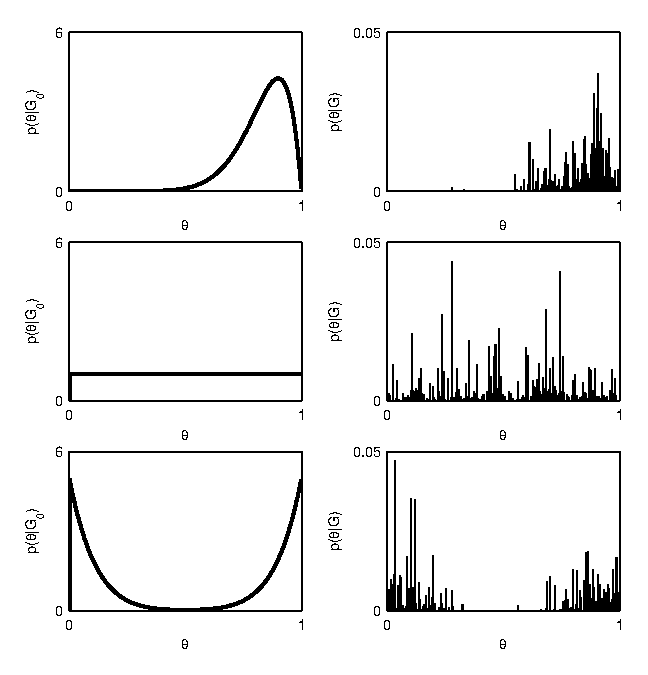
\epsfig{file=dpbase2.eps,width=10cm}
        \caption{Distributions sampled from a Dirichlet process with $\alpha=100$,
        and three different base distributions $G_0(\cdot)$. Base distributions are
        shown on the left, and sampled distributions are shown on the right. In the
        top line, the base distribution is Beta$(\cdot \condon 10,2)$, while in the
        middle row it is a uniform Beta$(\cdot \condon 1,1)$, while in the bottom
        row it is an equal mixture of a Beta$(\cdot \condon 10,1)$ and a
        Beta$(\cdot \condon 1,10)$.\efc}
        \label{dpbase}
        \end{center}
\end{figure}

\begin{figure}[t]
        \begin{center}
        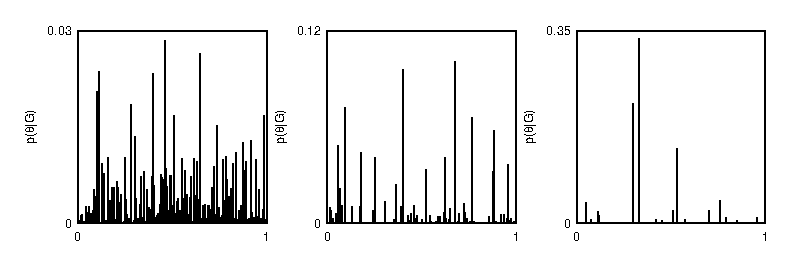
\epsfig{file=dpuniforms2.eps,width=14cm}
        \caption{Distributions sampled from a Dirichlet process with a uniform distribution
        over $[0, 1]$ as the base distribution $G_0(\cdot)$, and dispersion parameters
        of $\alpha=100$ (left), $\alpha=20$ (middle), and $\alpha=5$ (right). In all cases
        there are a countably infinite number of components (most of which are too small to
        see), but the distributions vary in the extent to which the probability mass is
        concentrated on a few points.\efc}
        \label{dpuniforms}
        \end{center}
\end{figure}

\subsection{Learning the Dispersion of Data}

A difficulty with Dirichlet process models, noted by Antoniak (1974), is that
it is usually too restrictive to specify a value of $\alpha$ {\it a priori}. The dispersion
parameter reflects the degree of variability in the parameter values, and is something
we would prefer to learn from data. In order to do so, we
first need to understand the relationship between the dispersion $\alpha$ and the
number of groups $k$ that will manifest among $n$ subjects. Note that $k$ now
refers not to the `true' number of groups, but to the number of manifest groups.
Antoniak (1974) shows that the probability $p(k \condon \alpha, n)$ that $k$
groups will be observed in $n$ samples from a model with a Dirichlet process
prior is
\begin{eqnarray}
        p(k \condon \alpha, n) &=& \frac{n!  \Gamma(\alpha)}{\Gamma(\alpha+n)}
        z_{nk} \alpha^k \nonumber \\
        &=& n \mathrm{B}(\alpha,n)  z_{nk} \alpha^k \label{prioronk} \\
        &\propto& z_{nk} \alpha^k, \nonumber
\end{eqnarray}
where $\mbox{B}(u,v)=\frac{\Gamma(u)\Gamma(v)}{\Gamma(u+v)}=
\int^1_0 \eta^{u-1}(1-\eta)^{v-1} d\eta$ is a standard
Beta function and  $z_{nk}$ is an unsigned Stirling number of the first kind.
The unsigned Stirling numbers count the number of  permutations of $n$ objects
 having $k$ permutation cycles (Abramowitz \& Stegun, 1972, pp. 824), and are found
by taking the absolute value of the corresponding signed Stirling numbers
$z_{nk}=|s_{nk}|$. There is no analytic expression for $s_{nk}$, but it is easily
calculated using the recurrence formula $s_{nk}=s_{n-1,k-1} - (n-1)s_{n-1,k}$,
and the special cases $s_{nn}=1$ for all $n$ and $s_{n0}=0$ for $n>0$. Note that
the use of $s$ and $z$ in this notation is unrelated to the previous use as the group
sizes and indices (the two uses will not come into conflict). Antoniak (1974) also
observes that the expected number of components sampled from a Dirichlet
process is given by,
\begin{eqnarray}
        E[k\condon \alpha, n] &=&
        \sum_{k=1}^{n} k \, p(k \condon \alpha, n)  \nonumber \\
        &=& \alpha \sum_{k-1}^n \frac{1}{\alpha + k -1} \nonumber \\
        &\approx& \alpha \ln\left(\frac{n+\alpha}{\alpha}\right).
        \label{kgrow}
\end{eqnarray}
Thus, although $k \rightarrow \infty$ with probability 1 as
$n \rightarrow \infty$ (Korwar \& Hollander, 1973), the number of components
increases in approximately logarithmically with the number of observations.
This is illustrated in Figure~\ref{dpgrow}a, which shows how the prior
over the number of components grows changes as a function of $n$, for a Dirichlet
process with $\alpha=10$.

\begin{figure}[t]
       \begin{center}
        \begin{tabular}{cc}
        Fixed $\alpha$ & Random $\alpha$\\
        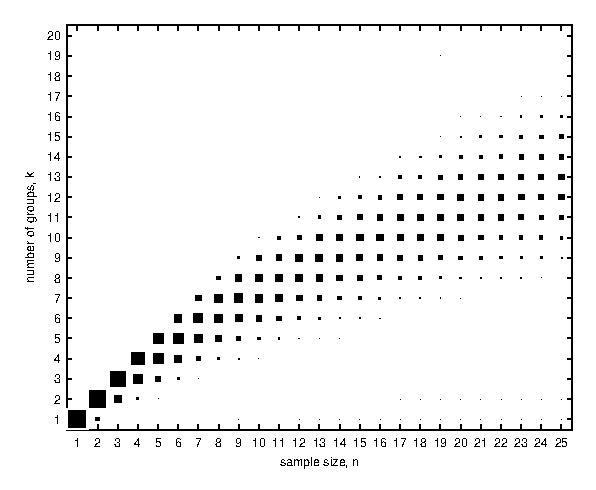
\epsfig{file=dpgrow.eps,width=7.5cm} &
        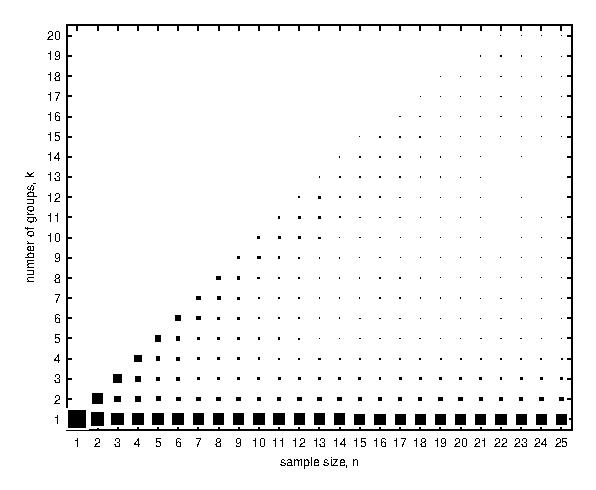
\epsfig{file=mixdpgrow.eps,width=7.5cm}\\
        (a) & (b)
        \end{tabular}
       \caption{\bfc
        Prior distributions over the number of components $k$ for sample sizes $n$
        ranging from 1 to 25. The panel on the left shows the prior for a Dirichlet process
        with dispersion $\alpha=10$, where the area of each rectangle is proportional
        to the probability associated with the corresponding value of $k$ for a given $n$.
        The panel on the right shows the marginal prior over $k$ for a Dirichlet process
        mixture in which the prior over $\alpha$ is a Gamma($\cdot \condon
        10^{-10}$, $10^{-10}$) distribution. \efc}
       \label{dpgrow}
       \end{center}
\end{figure}

In many contexts the dispersion $\alpha$ is unknown, so we specify a prior distribution
$p(\alpha)$,  allowing us to learn $\alpha$ from data. The resulting model is known as
a {\it Dirichlet process mixture}. Antoniak (1974) notes that the the posterior distribution
for $\alpha$ is influenced only by the number of distinct groups $k$, and not by the
details of the allocation of observations to those groups. Therefore, since
$p(k \condon \alpha, n)$  provides the likelihood function for $k$, we can apply
Equation~\ref{prioronk} to find the posterior distribution over $\alpha$ given some
observed data containing $k$ groups. Since the prior on $\alpha$ is not dependent on
the sample size $n$, we may write,
\begin{eqnarray}
        p(\alpha \condon k, n)
        &\propto& p(k \condon \alpha, n) \,  p(\alpha \condon n) \nonumber \\
        &=& p(k \condon \alpha, n) \,  p(\alpha) \nonumber \\
        &\propto& \mathrm{B}(\alpha,n) \,  \alpha^k \, p(\alpha). \label{agrow}
\end{eqnarray}
A common choice for $\prepost(\alpha)$ is the Gamma distribution
$\alpha \condon a,b \sim \mbox{Gamma}(\cdot \condon a,b)$ in which
$\prepost(\alpha) \propto \alpha^{a-1}e^{-b\alpha}$ (Escobar \& West, 1995).
If so, the posterior distribution becomes,
\begin{equation}
        \label{gampri}
        p(\alpha \condon k,n) \propto
        \alpha^{a+k-1} e^{-b\alpha} \, \mathrm{B}(\alpha,n).
\end{equation}
In particular, Escobar and West (1995) note that if we let  $a \rightarrow 0$ and
$b \rightarrow 0$ we obtain a so-called scale-invariant prior in which
$p(\alpha) \propto 1/\alpha$ (e.g., Jeffreys, 1961; Kass \& Wasserman, 1996).
However,
since this Gamma($\cdot \condon 0,0$) prior is improper, we have chosen to
approximate it with the proper but extremely similar prior Gamma($\cdot \condon
10^{-10}, 10^{-10}$). Figure~\ref{dpgrow}\panel{b} shows the marginal
prior over $k$ resulting from this choice of prior.

\section{Model Selection With Infinite Groups}

One benefit to the infinite groups model is the principled perspective
that it provides on the model order selection problem. Since model
order selection problems are commonplace in psychological modeling
(e.g., Landauer \& Dumais, 1997; Griffiths \& Steyvers, 2004;
Lee, 2001; Lee \& Navarro, 2005) it is worth discussing this point
in a little more detail.

When working with finite models, it is natural to think of $k$ as the
intrinsic model order. Every value of $k$ describes a different family
of distributions in Equation~\ref{finitegroups}, and so it is easy
to think of $k$ as defining a model $\mathcal{M}_k$ consisting of
all discrete distributions that consist of exactly $k$ point masses.
This means that, when inferring a finite group model to account for individual differences,
we need to address the model selection question of choosing a
model $\mathcal{M}_k$, and a parameter estimation problem in which
we pick a distribution $G(\cdot) \in \mathcal{M}_k$. From a Bayesian
standpoint (e.g., Wasserman, 2000) we would find a posterior distribution
over the models $p(\mathcal{M}_k \condon \vctr{x})$ and use this
to draw our inference about $k$. In order to find this posterior, we need
a prior distribution $p(\mathcal{M}_k)$. However, since it is not easy
to see how this prior might be chosen, it is quite common to use
 Bayes factors (e.g., Kass \& Raftery,  1995). This corresponds implicitly to the use of a uniform prior over
model orders, which may not be appropriate.\footnote{Note
that Lee and Webb's (in press) approach to finite group selection is a
little different to standard model order selection. Rather than placing
an implicit uniform prior over $k$, they use an implicit uniform prior
over the possible partitions of $n$ subjects.}
It seems unlikely, for example, that experimental data from 40 subjects---thus
requiring the consideration of model orders 1, 2, \ldots, 40---is equally as likely
to contain 23 different groups of subjects as it is to contain two different groups of subjects.

The infinite groups model takes a different view. By assuming that
the distribution $G(\cdot)$ has an infinite number of groups, we
no longer have any model classes to select between. In this framework,
we view $k$ as the \emph{variable} expression of $G(\cdot)$
through finite data. When we set a prior in this approach, it is
over the distributions themselves: A prior that we have derived from
basic considerations about the structure of the model. This, in turn,
\emph{implies} a prior over $k$ that reflects the rate at
which new groups are expected to appear when sampling from
$G(\cdot)$. At no point do we need to specify artificial model classes.
Moreover, since the natural way to think about inference
is to do posterior sampling over $G(\cdot)$, the number of observed
groups $k$ will emerge in inferring
$G(\cdot)$, rather than via a dedicated model selection
procedure.

\section{Modeling Discrete Data With Infinite Groups}

We now turn to the specification and application of the infinite groups model
to situations in which subjects provide discrete data. Suppose that
$n$ people perform some task in which $m$ possible responses can be
made on each trial, and the $i$th person experiences $r_i$ trials. We will specify a
simple cognitive model in which there is a multinomial distribution with
parameter vector $\vctr{\theta}_i = (\theta_{i1}, \ldots, \theta_{im})$
for the behavior of participant $i$. In this situation, the
natural way to describe data from the $i$th participant is with the vector
$\vctr{x}_i = (x_{i1}, \ldots, x_{im})$, in which $x_{ih}$ counts the number of
times that participant $i$ made response $h$. Note that this is a slight change
from the previous notation, since $\vctr{x}_i$ is now a vector of counts rather
than a list of the outcomes for every trial. Since our cognitive model is
multinomial, it is natural to use a Dirichlet distribution as the prior over $\vctr{\theta}_i$.
Specifically, we will assume a symmetric Dirichlet base distribution
with parameter $\beta$. This cognitive model, including the prior, is written
\[
       \begin{array}{rcl}
        \vctr{x}_{i} \condon \vctr{\theta}_i & \sim & \mbox{Multinomial}
        (\cdot \condon \vctr{\theta}_i) \\
        \vctr{\theta}_i \condon \beta & \sim & \mbox{Dirichlet}
        (\cdot \condon\beta).
       \end{array}
\]

If we now assume that each person belongs to one of an infinite number of
latent groups, we would incorporate an individual differences model by assuming
that each parameter value $\vctr{\theta}_i$ is drawn from some
discrete distribution $G(\cdot)$, and use the Dirichlet process to place a
prior over these distributions. However, since we do not wish to make strong
assumptions about the dispersion parameter $\alpha$, we use the Dirichlet process
mixture model in which we assume that $\alpha$ follows a
Gamma distribution. If we write this model using the stick-breaking
notation (as in Equation~\ref{infiniteprior}), we obtain the model
\begin{equation}
        \begin{array}{rcl}
        \vctr{x}_{i} \condon \vctr{\theta}_1, \ldots, \vctr{\theta}_\infty, g_i=z
        & \sim & \mbox{Multinomial}(\cdot \condon \vctr{\theta}_z) \\
        g_i \condon w_1, \ldots, w_\infty & \sim &
        \mbox{Multinomial}(\cdot \condon w_1, \ldots, w_\infty) \\
        w_1, \ldots, w_\infty \condon \alpha & \sim &
        \mbox{Stick}(\cdot \condon 1,\alpha) \\
        \alpha \condon a, b & \sim & \mbox{Gamma}(\cdot \condon a,b)\\
        \vctr{\theta}_z \condon \beta & \sim & \mbox{Dirichlet}(\cdot \condon\beta),
       \end{array}
        \label{idg}
\end{equation}
where the multinomial in the second line is of sample size 1.
The model is illustrated in
Figure~\ref{indivdiffs}. Performing inference in this infinite groups model
using the mixture of Dirichlet processes prior means being able to estimate
the joint posterior distribution $p(\vctr{g}, \vctr{\theta}, \alpha \condon
\vctr{x}, a, b, \beta)$. A straightforward Gibbs sampling scheme for drawing
samples from this posterior distribution is presented in the Appendix.
From these posterior samples we can construct estimates of the posterior
distribution itself using some density estimation technique (e.g.,
Hastie, Tibshirani \& Friedman, 2001, pp. 182--190).

Using this model to make inferences from data there are several
marginal posteriors that are of particular interest, corresponding to different
theoretical questions. Some examples include:
\begin{enumerate}
\item \label{q1} {\it How many groups?} This question corresponds to the model order
selection problem, by asking how many groups are manifest in the data. To answer this,
we want to know $p(k\condon \vctr{x})$, the
posterior probability that there are $k$ distinct groups in the
sample $\vctr{x}$. Notice that this is a property of the observed data, not an
inference about a population parameter. \vspace*{5pt}
\item {\it How dispersed is the population?} The complementary question to
(\ref{q1}) is to ask how groups might be distributed in the
population. Of course, in an infinite population it is not sensible to ask
how many groups exist.  The relevant distribution is $p(\alpha \condon \vctr{x})$,
the posterior distribution over the dispersion parameter. If most subjects
fall into a single group, then the posterior over $\alpha$ will place most mass
on small values, since the population is unlikely to be highly dispersed. \vspace*{5pt}
\item {\it What are the groups?} Clearly, in drawing inferences about the
sample we want to know not just how many groups there are, but also which people tend
to belong to the same groups. In this case, we want to know $p(\vctr{g} \condon \vctr{x})$.
In some cases, we might want to find the {\it maximum a posteriori} (MAP)
estimate for the group structure, namely $\hat{\vctr{g}} = \arg \max_{\vctr{g}}
p(\vctr{g} \condon \vctr{x})$. Alternatively, we might aim to get a sense for the
full distribution $p(\vctr{g} \condon \vctr{x})$ by finding specific groupings that
consistently appear in the posterior. \vspace*{5pt}
\item {\it What performance characterizes a group?} The original motivation for
proposing a groups model was to learn which subjects could be characterized
in the same way. Having inferred that some subjects belong to
the same group, we would like to know what parameter values of the cognitive model describe their
performance. In this case, we want to know $p(\vctr{\theta} \condon \vctr{x}, \vctr{g})$,
or some other summary measure for
this distribution such as $E[p(\vctr{\theta} \condon \vctr{x}, \vctr{g})]$.
\end{enumerate}

\begin{figure}[t]\begin{center}\epsfig{file=discreteinfgps.eps,width=9cm}
\caption{\bfc Dependencies in the \fcs  infinite groups model for discrete
data as it is used here. Shaded \fcs circles denote observed variables,
white circles are latent \fcs  variables, rounded squares \fcs denote
known parameter values, and plates indicate a set of independent
replications \fcs of the processes shown inside them. \efc}
\label{indivdiffs}\end{center}\end{figure}

\begin{figure}[t]
\begin{center}
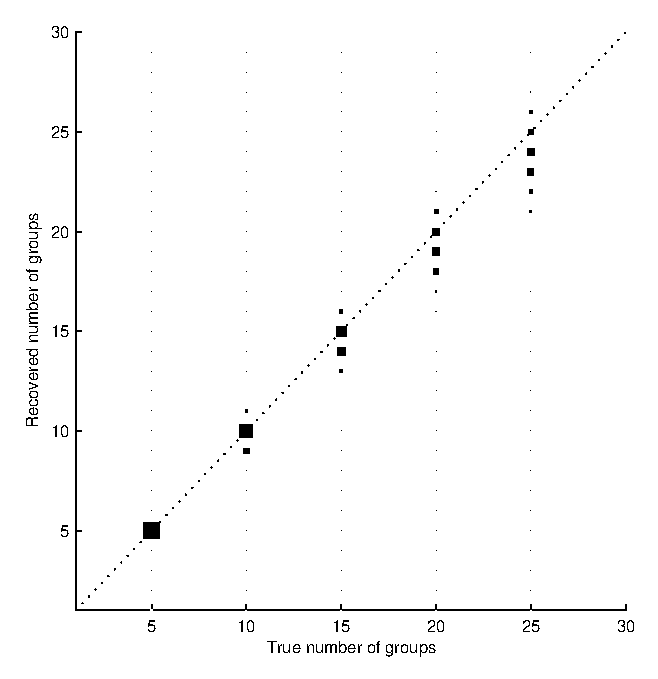
\epsfig{file=montecarlo.eps,width=10cm} \\
\caption{\bfc Simulations in \fcs which $n=100$ people provide $s=100$ observations
  each, and \fcs $m=20$ response options are possible on every trial.
 The true number of groups varies from 5 to 25. After a burn-in of only 500 samples,
and using only a single draw from the posterior distribution,
 the Gibbs sampler performs reasonably well.\efc}
\label{montecarlo}
\end{center}
\end{figure}

To provide a simple illustration of the performance of the model in the
context of the first question ``{\it how many groups?}'',
we created random data sets with $n=100$ people and
$r=100$ discrete observations per person, where each observation denotes a
choice of one of $m=20$ response options. The sample was divided into $k$
groups, and each group associated with a multinomial rate $\theta$ sampled
from a uniform distribution. People were allocated randomly to groups,
subject to the constraint that each group contained at least one member.
The number of groups in the data varied from 5 to 25, with 500 data sets generated
for each. For each data set, we ran the Gibbs sampler for 500 iterations and
then drew a single sample from the posterior distribution. Figure~\ref{montecarlo}
plots the distribution over the recovered number of groups as a function of the
true number of groups represented in the data. Inspection of this figure shows that,
for the most part, the Gibbs sampler recovers the appropriate number of groups in
the data. There is a slight tendency to underestimate the number of groups in
some cases, but as argued by Kontkanen et al.\ (2005), this is not undesirable
behavior when extracting a partition, since it generally reflects ``different''
groups with parameter values so similar that they cannot be distinguished without
much more data. Erring on the side of simpler models would appear to be the right
thing to do in this situation.

\section{Individual Differences in Categorization}

\begin{figure}[t]
\begin{center}
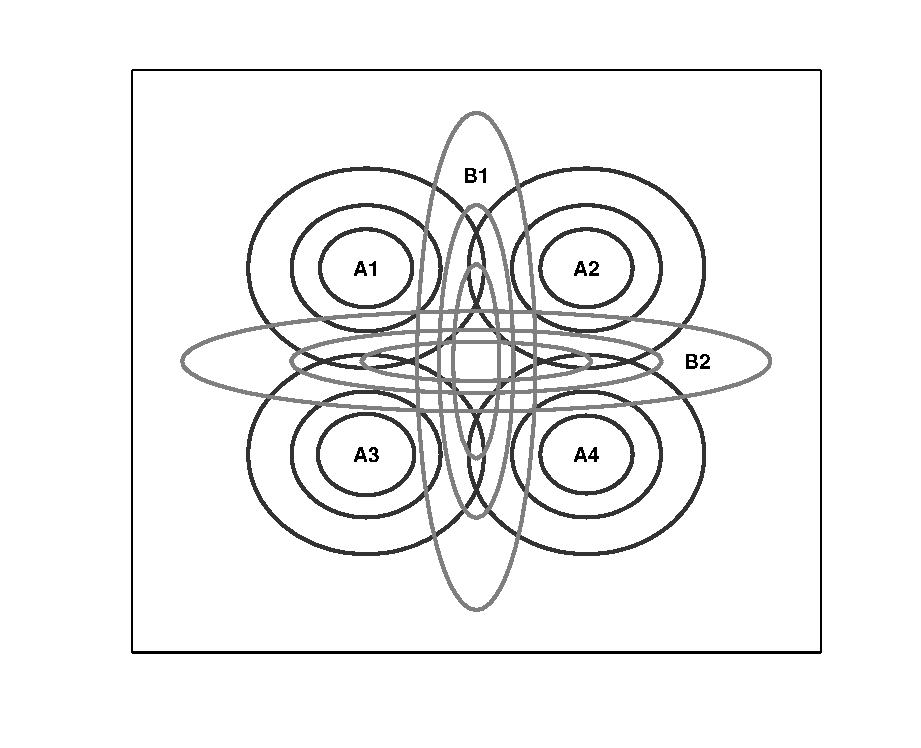
\epsfig{file=catmix.eps,width=11cm}
\caption{\bfc The category densities \fcs used in McKinley and Nosofsky's
(1995) experiment 2. Category A (dark grey) \fcs is a mixture of four
Gaussians, while category B (light grey) \fcs is a mixture of two
Gaussians. The 30\%, 60\% and 90\% confidence ellipses are shown for
each of the six densities. \efc}
\label{catpic}
\end{center}
\end{figure}

We now present an application of the infinite groups model.
An elegant category learning experiment by McKinley and Nosofsky (1995)
investigated 10 people's\footnote{McKinley and Nosofsky (1995) actually
report data for 11 subjects. However, the data currently available
to us include only 10 of these.} ability to discriminate between the two
probabilistic categories shown in Figure~\ref{catpic}. The stimuli were
circles with a radial line running through them, and so the two dimensions
depicted in Figure~\ref{catpic} correspond to the radius of the circle,
and the angle of the line. Category A (dark grey) is a mixture of four
Gaussian distributions, while category B (light grey) is a mixture of two
Gaussians. On any given trial in the experiment, a stimulus was sampled
from one of the six Gaussian distributions. Subjects were asked whether
it came from category A or category B, and provided feedback as to the
accuracy of their response. Because the categories are inherently probabilistic
and the category densities are quite complicated, this task is very difficult,
and shows evidence of differences not only during the course of category
learning, but in the final structures learned.

In order to learn about the variation between subjects, we applied the
infinite groups model to the data from this experiment. In doing so, we
were interested in how the subjects' classification performance varied
as a function of the \emph{source}. For the $i$th participant we obtain
the data vector
$\vctr{x}_i=\left(x_i^{(A_1)}, x_i^{(A_2)}, x_i^{(A_3)}, x_i^{(A_4)},
x_i^{(B_1)}, x_i^{(B_2)} \right)$
in which $x_i^{(l)}$ records the number of correct responses to stimuli
generated from distribution $l$. We are also given a vector of sample
sizes,
$\vctr{r}_i=\left(r_i^{(A_1)}, r_i^{(A_2)}, r_i^{(A_3)}, r_i^{(A_4)},
r_i^{(B_1)}, r_i^{(B_2)} \right)$
indicating how many trials of each type appeared in each subjects' data.
The natural thing to model is the probability of making the correct response to
stimuli sampled from each of the six components.  So the model would
model would predict that for the $i$th participant, $p(\mbox{Correct}
\condon \mbox{Sample from } A_1) = \theta_i^{(A_1)}$. The cognitive
model therefore describes binomial distributions, so that if the $i$th
participant belongs to group $z$,
\[
       x_i^{(l)} \condon r_i^{(l)}, \theta_z^{(l)}, g_i=z  \sim
        \mbox{Binomial}\left(\cdot \condon \theta_z^{(l)}\right)
\]
for all $l \in (A_1, A_2, A_3, A_4, B_1, B_2)$, and where the binomial
is of sample size $r_i^{(l)}$. Group $z$ would therefore
have the parameter vector
$\vctr{\theta}_z=\left(\theta_z^{(A_1)},
\theta_z^{(A_2)}, \theta_z^{(A_3)}, \theta_z^{(A_4)}, \theta_z^{(B_1)},
\theta_z^{(B_2)}\right), $
where each element of this vector is a binomial rate. The fact that we have specified
a multidimensional space for $\vctr{x}$ and $\vctr{\theta}$ has no bearing on the
stick-breaking prior over $\vctr{w}$, so it is still appropriate to write the infinite
discrete groups model as
\[
        \begin{array}{rcl}
        g_i \condon w_1, \ldots, w_\infty & \sim &
        \mbox{Multinomial}(\cdot \condon w_1, \ldots, w_\infty) \\
        w_1, \ldots, w_\infty \condon \alpha & \sim &
        \mbox{Stick}(\cdot \condon 1,\alpha) \\
        \alpha \condon a, b & \sim & \mbox{Gamma}(\cdot \condon a,b).\\
        \end{array}
\]
The only modification that we need to make is to specify a multidimensional base
distribution $G_0(\cdot)$. To do so, we assume that each of the binomials has the same
symmetric Beta prior, implying that
\[
        \begin{array}{rcl}
        \theta_{z}^{(l)} & \sim & \mbox{Beta}(\cdot \condon \beta),
        \end{array}
\]
for all $l \in (A_1, A_2, A_3, A_4, B_1, B_2)$.

\begin{figure}[t]
\begin{center}
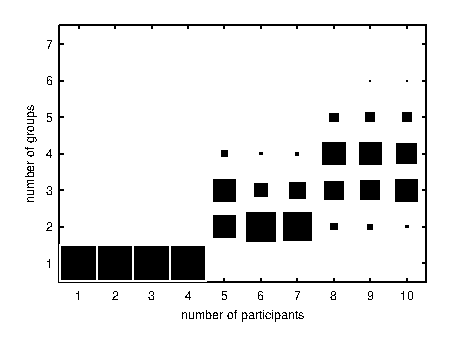
\epsfig{file=catgrow.eps,width=8cm}
\caption{Estimated posterior over $k$ as a function of $n$. Assuming subjects
arrive in a fixed order, from the first to the tenth person, we can see that the
number of inferred groups changes as more people are observed. The area of the
squares is proportional to the posterior probability of $k$ given $n$. \efc}
\label{catgrow}
\end{center}
\end{figure}

\begin{figure}[t]
\begin{center}
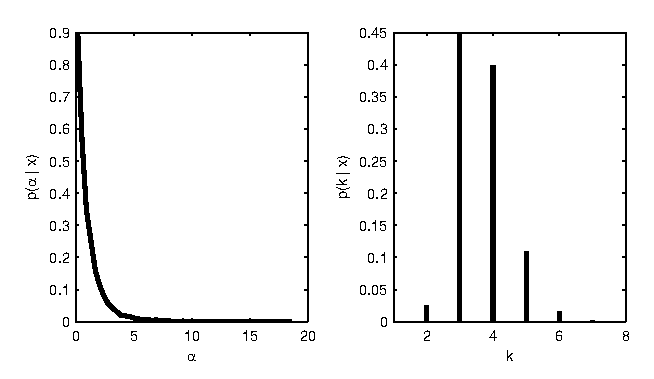
\epsfig{file=mn2_300.eps,width=10cm}
\caption{\bfc Estimated posterior distributions \fcs over $\alpha$ and $k$
when the infinite groups model is applied to \fcs McKinley and Nosofsky's (1995)
experiment 2.\efc}
\label{mn2}
\end{center}
\end{figure}

\begin{table}[t]\begin{center}
\caption{\bfc Estimated probability with which \fcs subjects in
McKinley and Nosofsky's (1995) experiment \fcs 2 belong to the same
group. For visual clarity, the probabilities are given as percentages.}
\label{covar}
\protect\footnotesize \vspace*{5pt}
\begin{tabular}{c|cccccccccc}
&1&2&3&4&5&6&7&8&9&10 \\  \hline
1&&37&0&73&0&58&68&36&43&55 \vspace*{-5pt}\\
2&&&22&34&1&68&56&3&5&67 \vspace*{-5pt}\\
3&&&&1&57&1&0&0&0&2 \vspace*{-5pt}\\
4&&&&&0&44&52&53&60&43 \vspace*{-5pt}\\
5&&&&&&0&0&0&0&0 \vspace*{-5pt}\\
6&&&&&&&86&4&7&93 \vspace*{-5pt}\\
7&&&&&&&&11&16&86 \vspace*{-5pt}\\
8&&&&&&&&&91&4 \vspace*{-5pt}\\
9&&&&&&&&&&7 \\
\end{tabular}
\vspace*{10pt}
\protect\normalsize
\end{center}\end{table}

For each of the 10
subjects we used only the last 300 trials of the experiment, in order
to look for differences in the learned category structure, rather than
differences in the learning process itself. In order to conduct a Bayesian
analysis, we set principled \emph{a priori} parameter values rather than
fitting the model to the data. Since we know that both responses (i.e.,
``$A$'' and ``$B$'') are possible but are otherwise ``ignorant'', the natural
choice for the base distribution is the uniform distribution (see Jaynes,
2003, pp.\ 382--386), which is obtained by setting $\beta=1$, and since
we have no strong beliefs about $\alpha$ we would like a scale-invariant
prior (see Jeffreys, 1961) in which $a \rightarrow 0$, $b\rightarrow 0$.
Once again, in order to ensure a proper prior, we chose $a=b=10^{-10}$
as a compromise between ignorance and propriety. To approximate
the posterior distribution over $\alpha$, $k$ and other relevant
parameters, we used the Gibbs sampler to draw 10,000 samples from
the joint posterior distribution (after an initial burn-in period of 1,000
iterations), with a lag of 5 iterations between samples to minimize
autocorrelation between samples.
\begin{figure}[t]
\begin{center}
\begin{tabular}{cc}
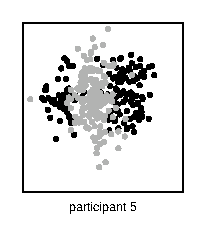
\epsfig{file=cp1.eps,width=5cm} & 
\epsfig{file=cp2.eps,width=5cm} \\
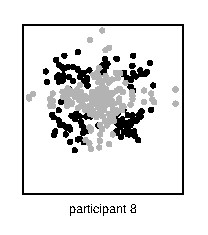
\epsfig{file=cp3.eps,width=5cm} & 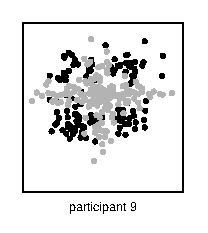
\epsfig{file=cp4.eps,width=5cm}
\end{tabular}
\caption{\bfc Last 300 trials for subjects \fcs 5, 7, 8
  and 9 in McKinley and Nosofsky's (1995) experiment 2. \fcs Black dots
  denote ``A'' responses, and grey dots denote ``B'' responses. \efc}
\label{indivs}
\end{center}
\end{figure}

We first consider the question of selecting the model order ({\it ``how many
groups?''})  by
examining how the distribution $p(k \condon \vctr{x})$ changes as a
function of $n$. To do this, we imagine that the 10 subjects entered
the lab in order of participant ID. Figure~\ref{catgrow} shows how the
posterior distribution over $k$ changes as more subjects are observed:
the model grows with the data. Initially there is evidence for only a
single group, but once the 10th participant is observed, there is strong
evidence for about 3 or 4 groups. The last of these posterior distributions
(in the case when $n=10$) is illustrated in Figure~\ref{mn2}b.
We can also use our samples to ask about the amount of variability that
we believe exists in the population ({\it ``how much dispersion?''}).
Figure~\ref{mn2}a shows the estimated posterior density
 $p(\alpha \condon \vctr{x})$, which indicates a strong preference
for smaller values of $\alpha$. However, with such a small sample
size, this distribution still reflects the near-ignorance
prior that we chose for this analysis.

Turning now to the third question  ({\it ``what are the groups?''}), the
small number of subjects allows us to present a nice summary of
the behavior of the posterior distribution $p(\vctr{g} \condon \vctr{x})$.
To do so,
Table~\ref{covar} shows the estimated (marginal) posterior probability
that any two subjects belong to the same group. This table reveals a
rich pattern of similarities and differences, indicating that the relationships
between subjects is not arbitrary. To illustrate this, we
turn to a characterization of the groups
themselves ({\it ``what performance?''}). For these data, it is most
informative to plot some of the raw data rather than report parameter
values, because the data have a natural two-dimensional graphical
structure while the parameters are naturally six-dimensional.
Figure~\ref{indivs} plots the last 300 stimuli observed by subjects
5, 7, 8 and 9, and the decisions that they made. Broadly speaking,
participant 5 is sensitive only to variation along the $x$-axis, participant
7 is sensitive only to variation on the $y$-axis, while subjects 8 and
9 do a good job of learning the category structures on both dimensions.
As a result, subjects 5 and 7 rarely appear in the same group as one
another or with subjects 8 and 9 (with probabilities ranging from 0\%
to 7\%), while subjects 8 and 9 almost always (91\%) co-occur.
In other words, the relational structure implied by Table~\ref{covar}
reflects the qualitative individual differences that are apparent from
visual inspection of Figure~\ref{indivs}.

\section{Individual Differences Among Psychologists}

Another application of the infinite groups model regards the publication
habits of psychologists. As an initial investigation, we took the publication
lists posted on the websites of staff in psychology departments at the
following six institutions: Boston College, Cardiff University, Johns Hopkins
University, The University of Edinburgh, Florida Atlantic University
and Colorado State University. This yielded a total of 125 academics
publishing in 254  outlets\footnote{The original data set contained 508
outlets, but half of them were missing from the analyzed data set due to a
corrupted file.}. Since most academics list only recent or selected publications,
the data represent a subset of publication behavior that people prefer to
announce. The distribution of the number of listed publications per
academic was highly skewed (the skewness was 5.25), with a median value
of 7 and an interquartile range of 10.5.

\begin{figure}[t]
\begin{center}
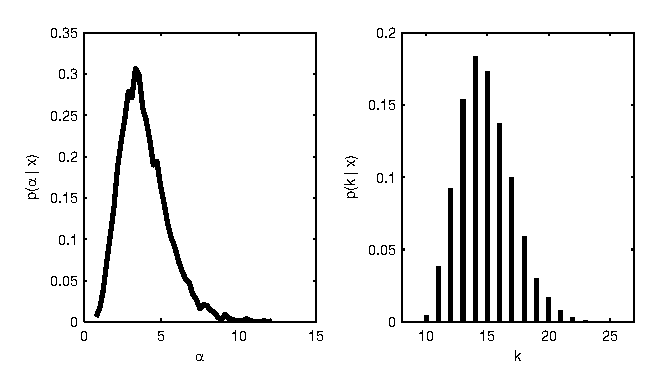
\epsfig{file=pubdist.eps,width=10cm}
\caption{\bfc Estimated posterior distributions \fcs over $\alpha$ and $k$
when the infinite groups model is applied to the publications data.\efc}
\label{pubdist}
\end{center}
\end{figure}

Using the infinite groups model, we would like to learn the patterns of
similarity and difference in declared publication preferences among these
authors. The model in this case is straightforward version of the usual
infinite groups model, with a single group corresponding to a multinomial
distribution over the 254 outlets. Again, we start only with the belief that any
author is able to publish in any outlet, implying that $\beta=1$. Not knowing
anything \emph{a priori} about the dispersion, we set the prior by setting
$a=b=10^{-10}$. After an initial burn-in period of 1000 samples to ensure that
the Gibbs sampler had converged, we drew 10,000 samples from the posterior
distribution over groups, with a  lag of 5 iterations between samples. The
resulting posterior distributions over $\alpha$ and $k$ are shown in
Figure~\ref{pubdist}, and suggest that there are most likely between 12 and
17 groups in these data.

One difficulty with the analysis of these data is that the full posterior distribution over
group assignments cannot be displayed easily. In order to provide insight
into the structure that the infinite groups model extracts from these data, we
undertook the following analysis. We took a set of ten successive samples (again, with
a lag of five) from the Markov chain used to produce Figure~\ref{pubdist}, and averaged
across the corresponding ten partitions to find an estimate for the expected probability
with which each academic belongs to each group. In order to interpret the groups, we
can list the names of the people that are expected to belong to them. Alternatively, we can
find the ``prototypical performance'' associated with each group. In this case, we can
calculate the expected probability with which a group member publishes
in a particular journal. A simple way of interpreting the groups is to provide a list
of typical journals for each group,  since journal names are highly informative,
whereas the author names often are not.

\begin{table}[p]
        \begin{center}
        \caption{Prototypical journals for the five most prominant author-clusters.
        The rankings are based on data that are normalized for the base rates
        of both journals and authors. All five represent structures that are found
        across most of the posterior distribution.}
        \label{jnls} \footnotesize
        \begin{tabular}{l}
        \\ {\bf 1. Cognitive Psychology} \\ \hline
        Journal of Experimental Psychology: Learning, Memory \& Cognition \tbsp \\
        Journal of Experimental Psychology: Human Perception \& Performance \tbsp \\
        Brain \& Language  \tbsp \\
        Perception \& Psychophysics \tbsp \\
        Quarterly Journal of Experimental Psychology   \tbsp \\
        \\  {\bf 2. Behavioral Psychology} \\ \hline
        Journal of Experimental Psychology: Animal Behavior Processes  \tbsp  \\
        Quarterly Journal of Experimental Psychology\tbsp \\
        Journal of the Experimental Analysis of Behavior  \tbsp  \\
        Behavioral Neuroscience  \tbsp  \\
        Applied Ergonomics \tbsp \\
        \\  {\bf 3. Social Psychology} \\   \hline
        Journal of Personality \& Social Psychology   \tbsp  \\
        Personality \& Social Psychology Bulletin\tbsp  \\
        Cognition \& Emotion  \tbsp   \\
        Social Cognition \tbsp \\
        The Behavioral \& Brain Sciences  \tbsp   \\
        \\ {\bf 4. Developmental Psychology} \\ \hline
        Developmental Psychology    \tbsp \\
        Journal of Experimental Child Psychology  \tbsp  \\
        Developmental Review  \tbsp  \\
        Infant Behavior and Development   \tbsp \\
        Learning \& Individual Differences   \tbsp  \\
        \\      {\bf 5. Medicine \& Differential Psychology} \\ \hline
        Personality \& Individual Differences   \tbsp \\
        Intelligence    \tbsp  \\
        Diabetic Medicine  \tbsp \\
        British Medical Journal \tbsp  \\
        Diabetes Care   \tbsp \\
        \end{tabular}
        \normalsize
        \vspace*{10pt}
        \end{center}
\end{table}

Note that this is a rather different analysis to the one we would obtain if we
partitioned the journals themselves. In this case we are interested in groups
of people, and measure their common behavior in terms of the journals
they publish in. This does not necessarily produce partitions of journals,
however, since multiple groups of people may use the same journal. In short,
the idea is we want groups of authors because we are interested in their individual
differences: in this analysis, journal usage is the ``parameter'' for a group of
authors, rather than the other way around. We should also mention the reason
for using a small number of nearby samples. In this analysis, we want to
partially preserve the autocorrelation between samples. This is because the
full posterior distribution is likely to be multimodal, and while ``local averaging''
across samples from the same peak is likely to be beneficial, averaging across
samples from different peaks would likely corrupt the analysis. We repeated
this procedure across a large number of randomly chosen locations in the
Markov chain, and looked for stable clusters of authors, defined as those
that produced strong agreement in the rank ordering of journals.

Table~\ref{jnls} shows the top five journals for the five most prominant
groups found in the posterior distribution. As indicated by the labels,
four of the five groups have a very natural interpretation in terms of sub-fields
within the discipline, namely cognitive, behavioral, social and developmental
psychology. The fifth group contains journals that are representative
of both medical research  (e.g., {\it Diabetic Medicine} and {\it British
Medical Journal}) and differential psychology (e.g., {\it Intelligence} and
{\it Personality \& Individual Differences}). While there is a possibility
that this reflects a broader correlation in the interests of psychologists, it
seems more likely that this cluster  results from the multiple interests of
some members of our sample.

\section{Individual Differences in Web Browsing}

\begin{table}
\begin{center}
\caption{Categories for the MSNBC.com web pages.}
\label{weblabels}
\begin{tabular}{lll}
\\ \hline
1. Front Page & 7. Miscellaneous & 13. Summary \tbsp \\
2. News & 8. Weather & 14. Bulletin Board Service \tbsp\\
3. Technology & 9. Health & 15. Travel \tbsp\\
4. Local & 10. Living & 16. MSN-News\tbsp\\
5. Opinion & 11. Business & 17. MSN-Sport \tbsp\\
6. On-Air & 12. Sports & \\
\hline
\end{tabular}
\vspace*{10pt}
\end{center}
\end{table}

The final application considers the behavior of 1000 people browsing
on MSNBC.com and news-related portions of MSN.com
on September 28, 1999. Rather than record every webpage viewed,
each page is classified using one of the 17 categories
listed in Table~\ref{weblabels}, such as ``news'', ``technology'' and
``health''. For every user the data count the number of times they
visited pages belonging to each of the categories. The number of webpages
that belonged to each category varied from 10 to 5000. This data set is
taken from a much larger public database that records the behavior
of all 989,818 (anonymous) users that visited MSNBC.com on that day,
previously analyzed in some detail by Cadez et al.\ (2003).

One reason for considering these data is that they represent the unconstrained
behavior of people engaged in a natural task. The analysis of large, natural
data sets is not a standard approach in cognitive psychology which has
traditionally been dominated by the experimental method. Although generally
effective, this approach tends to restrict the domain of psychology to simplistic,
often implausible contexts. As a complementary approach, analyzing large
data sets collected in rich environments provide a reflection of real-world
behavior and decision-making. By applying cognitive models in such contexts,
we may obtain insights that are not easily obtained in the laboratory.

To analyze these data using the infinite groups model, we group visitors to the site by
the frequencies with which they visit each of the 17 categories of websites. Once again,
the cognitive model is a multinomial over the 17 categories, and we want to find
groups of people who have the same multinomial. To do so, we again assume that
$\beta=1$ and $a=b=10^{-10}$. After a burn-in of 1000 samples, we again drew
10,000 samples from the posterior $p(\vctr{g} \condon \vctr{x})$ with a lag of 5
iterations between samples. The posterior distributions over $\alpha$ and $k$ are
shown in Figure~\ref{webdata}, and suggest that there are approximately 40 different
groups represented among these 1000 people. In order to provide an interpretable summary
of the full posterior over groups, we repeated the analysis used in the last section, in
which we associate groups with an ``expected performance profile''. In this case, we find
the expected distribution over the 17 categories for each different group. However, since
there is a great deal of uncertainty about the make-up of many of the groups, we
restrict the analysis to a few of the prominent and consistent groups.

\begin{figure}[t]
\begin{center}
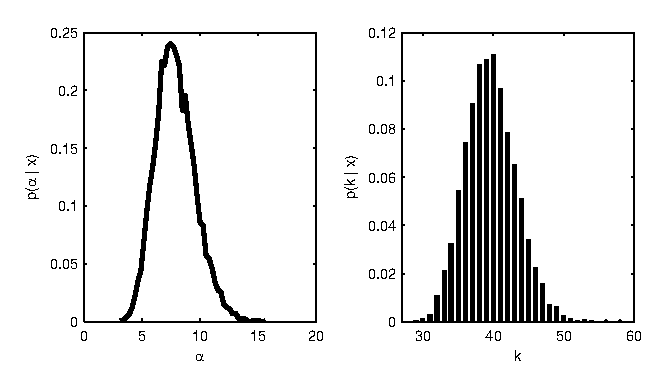
\epsfig{file=webdata.eps,width=10cm}
\caption{\bfc Estimated posterior distributions \fcs over $\alpha$ and $k$ when the
infinite groups model is applied to the web data.\efc}
\label{webdata}
\end{center}
\end{figure}

As with the publication data, there is evidence for stable groupings of people. Across most
of the posterior distribution we observe the three groups illustrated on the left hand side
of Figure~\ref{webclus}. In each case, there is a group of people who visit only one type
of web page, either ``front page'', ``summary'' or ``weather''. Given the extremely tight
focus of these distributions, we might safely conclude that these people were engaged in
very specific searches. Their interactions with the web environment were presumably oriented
towards a very specific objective (e.g., find a weather report). On the other hand, there is some
evidence for groups such as those illustrated on the right hand side of Figure~\ref{webclus}.
In these cases, people visited a range of different pages, particularly ``front page'', ``news'',
``technology'' and ``on-air'' pages. Distributed patterns of hits such as these suggest a
different interpretation of user behavior. In these cases, people appear to be engaged in
exploratory search through the web environment (i.e., genuinely ``browsing'' rather than simply
``looking-up'').

\begin{figure}[p]
\begin{center}
\scriptsize
\begin{tabular}{cc}
\hspace*{-20pt}  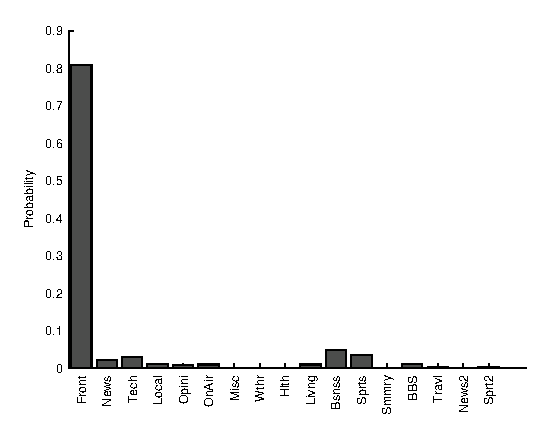
\epsfig{file=web_front.eps,width=8cm} \tbsp
&  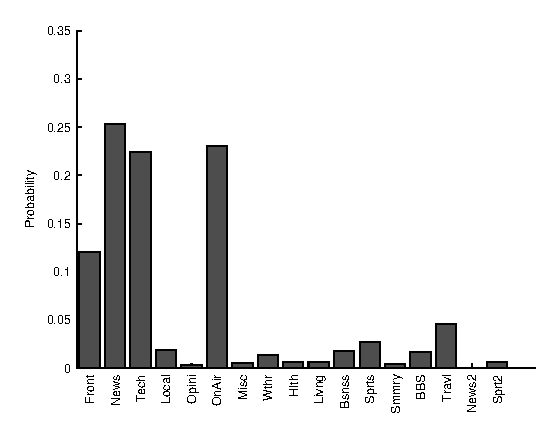
\epsfig{file=web_frontnewstechonair.eps,width=8cm} \\
\hspace*{-20pt}  (a)&(d)\\
\hspace*{-20pt}  \epsfig{file=web_summary.eps,width=8cm}  \tbsp
&  \epsfig{file=web_frontnewstechonair2.eps,width=8cm} \\
\hspace*{-20pt}  (b) &(e)\\
\hspace*{-20pt}  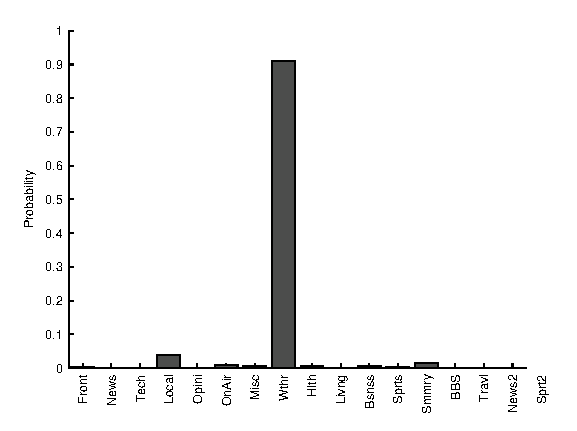
\epsfig{file=web_weather.eps,width=8cm} \tbsp
&  \epsfig{file=web_frontnewstechlocalbbs.eps,width=8cm} \\
\hspace*{-20pt}  (c) & (f) \\
\end{tabular}
\caption{\bfc Six different groups observed in the web data. In the three groups shown
on the left, people visited only one type of page, either ``front page'',
``summary'' or ``weather''. All three groups on the right show a consistent
tendency to visit ``front page'', ``news'', ``technology'' and ``on-air'' pages,
but with different relative frequencies in each case.
In addition, group (f) also shows interest in ``health'' and ``bulletin
board'' pages.\efc}
\label{webclus}
\end{center}
\normalsize
\end{figure}

There is a great deal of variety in the kinds of exploratory browsing patterns
observed across the posterior distribution.
An exploratory analysis suggests that the clustering of ``front page'',
``news'' and ``technology'' pages is highly stable, in the sense that across most of the
posterior there exist large groups that assign high probability to all three categories.
However, there is a considerable degree of (apparently smooth) variation
in the relative interest in these three topics. This is illustrated in the comparison between
panels d and e in Figure~\ref{webclus}, which show the same qualitative pattern
of preferences, but display subtle differences in the various probabilities.
Moreover, when we consider panel f, the same ``clumping'' of
 ``front page'', ``news'', ``technology'', is observed, but with the
addition of ``local'' and ``bulletin board service'' instead of ``on-air''.
Finally, there is some variation across the full posterior distribution in terms
of the kinds of patterns it identifies.

Taken together, these results suggest that, while the infinite groups model is
highly successful at identifying the focused search behavior illustrated on the
left hand side of Figure~\ref{webclus}, the more complex variation in exploratory
browsing behavior is only captured in part. The apparently smooth variation
from panel d to panel e suggests that a more complete account of individual
differences in web browsing may require multimodal and continuous parameter
distributions. The fact that there are similarities between panel d and panel f, for
instance, suggests that we may need to explore models that allow structured
relationships between groups.

\section{General Discussion}

Cognitive models aim to describe and predict how people think and act. Since
different people think and act in different ways, we require models that allow us
to learn complicated patterns of
variation. The individual differences framework outlined
in this paper provides a powerful method of representing the similarities
and differences between people. By using a group model we can
capture multimodality in individual differences, thereby remaining
sensitive to the possibility of qualitative differences in performance. By
adopting the Dirichlet process prior, we are able to view observed groups not as
 a fixed structure that fully explains the variation between individuals,
but rather as representatives of a latent, arbitrarily rich structure.
Additionally, by placing a prior over the dispersion we are able to learn about the extent of the
the variability itself.

Our approach could be extended in a number of ways, enabling
us to capture a greater range of individual differences phenomena.
One very simple extension would be to generalize the Dirichlet process prior
to other stick-breaking priors. As Ishwaran and James (2001) note, this family
is quite general, incorporating the Poisson-Dirichlet process
(Pitman \& Yor, 1997) and Dirichlet-Multinomial processes (Muliere \& Secchi, 1995)
among others.
Alternatively, one might choose to move beyond priors over the discrete distributions,
instead using a  different class of nonparametric priors, one that
covers continuous  distributions such as P\'{o}lya trees (Kraft, 1964; Ferguson, 1974)
or Dirichlet diffusion trees (Neal, 2003).

A  different extension to the framework can be motivated by returning to
the unlucky numbers experiment. In this example
 there is an issue regarding how to treat the one person who
responds 86. Does this person belong with the ten people who said 87?
It may be the case that this person is not a cricket fan, and is a representative
of a genuinely new group (fans of Agent 86 in the TV show {\it Get Smart},
perhaps). It is difficult to distinguish these cases, particularly since
group models are rather unforgiving in their requirement that all group members
share the same parameter value. One of the merits of the stochastic
parameters approach is that it allows some smooth variation. If our data consisted
only of cricket fans, a stochastic parameters model would  learn an individual
differences distribution centered on 87, since this is the typical behavior, but
allow some variability to be expressed.
However, once we reintroduce the  13 group and the 4 group, a unimodal stochastic
parameter model will be inadequate.

A natural solution to this problem would be to build individual differences models
that capture the strengths of both frameworks. One approach would be to adopt
an {\it infinite stochastic groups model}, which would produce multimodal continuous
distributions by convolving each point mass with a  continuous distribution.  In this
approach, we would assume that there are distinct groups
of subjects in our data, as with the infinite groups approach. However, within a group we
would allow there to be continuous, unimodal
variation, as with the stochastic parameters approach. Indeed,
one of the reasons that we have avoided conducting some sort of competition
between the different frameworks is that they are designed to address different
phenomena. Accordingly, we feel that the better approach is to pursue more powerful
modeling frameworks that integrate the best features of each.

Another direction for future work would be to allow structured relationships
between groups. One possibility would be to postulate a separate Dirichlet process
prior over each parameter. Alternatively, we could use a hierarchical Dirichlet process
(Teh,  Jordan, Beal \& Blei, 2004), in which the distribution sampled from a Dirichlet process is itself
a Dirichlet process. Finally, we may wish to consider an {\it idiosyncratic strategies model},
in which it is assumed that all subjects draw on a common set of strategies
 but combine them in an unique way (e.g., Girolami \& Kab\'{a}n, 2004). In short,
the infinite groups model is not by itself an authoritative account of individual differences.
Rather, it is a representative of a large class of flexible models, each suggesting a fruitful
approach for the development of powerful new cognitive models of individual differences.

\section*{Acknowledgements}
Correspondence address: Daniel Navarro, Department of Psychology, University of
Adelaide, SA 5005, Australia. E-mail: daniel.navarro@adelaide.edu.au, Tel.:
+61 8 8303 5265, Fax.: +61 8 8303 3770. This research was supported by Australian
\acs Research Council grant DP-0451793. We thank Yves Rosseel
for \acs providing a copy of the categorization data, Victoria Dennington for collecting
the publication data, as well as MSNBC and the UCI KDD archive
(http://kdd.ics.uci.edu/) for making the web data available. We would also like to thank
Jeff Rouder, E. J. Wagenmakers and an anonymous reviewer for helpful comments,
and Hemant Ishwaran for providing some useful pointers.

\section*{References}
\begin{list}{}{\setlength{\leftmargin}{12pt}\setlength{\itemindent}{-12pt}\setlength{\parsep}{0pt}}
\item Abramowitz, M. \& Stegun, I. A. (1972). {\it Handbook of Mathematical Functions with Formulas, Graphs, and Mathematical Tables}. New York: Dover.
\item Aldous, D. J. (1985). Exchangeability and related topics. In P. L. Hennequin (Ed.) {\it \'{E}cole d'\'{E}t\'{e} Probabilit\'{e}s de Saint-Flour XII.} Springer-Verlag.
\item Anderson, J. R. (1990). {\it The Adaptive Character of Thought}. Hillsdale, NJ: Lawrence Erlbaum.
\item Anderson, J. R. (1991). The adaptive nature of human categorization. {\it Psychological Review, 98}, 409-429.
\item Antoniak, C. E. (1974). Mixtures of Dirichlet processes with applications to Bayesian nonparametric problems. {\it Annals of Statistics, 2}, 1152-1174.
\item Ashby, F. G., Maddox, W. T. \& Lee, W. W. (1994). On the dangers of averaging across subjects when using multidimensional scaling or the similarity-choice model. {\it Psychological Science 5}, 144-151.
\item Bernardo, J. M. \& Smith, A. F. (2000). {\it Bayesian Theory}. New York: Wiley.
\item Blackwell, D. (1973). Discreteness of Ferguson selections. {\it Annals of Statistics, 1}, 356-358.
\item Blackwell, D. \& MacQueen, J. B. (1973). Ferguson distributions via P\'{o}lya urn schemes. {\it Annals of Statistics, 1}, 353-355.
\item Blei, D. M., Ng, A. Y. \& Jordan, M. I. (2003). Latent Dirichlet allocation. {\it Journal of Machine Learning Research, 3}, 993-1022.
\item Blei, D. M., Griffiths, T. L., Jordan, M. I. \& Tenenbaum, J. B. (2004). Hierarchical topic models and the nested Chinese restaurant process.  In S. Thrun, L. Saul, and B. Sch\"{o}lkopf (eds), {\it Advances in Neural Information Processing Systems 16}. Cambridge, MA: MIT Press.
\item Buntine, W. L. (1994). Operations for learning with graphical models, {\it Journal of Artificial Intelligence Research, 2}, 159-225.
\item Cadez, I. V., Heckerman, D., Meek, C., Smyth, P. \& White, S. (2003). Model-based clustering and visualization of navigation patterns on a Web site, {\it Journal of Data Mining and Knowledge Discovery, 7}, 399-424.
\item Chen, M., Shao, Q. \& Ibrahim, J. G. (2000). {\it Monte Carlo Methods in Bayesian Computation}. New York: Springer.
\item Cowles, M. \& Carlin, B. (1996). Markov Chain Monte Carlo convergence diagnostics: A comparative review.{\it Journal of the American Statistical Association, 91}, 833-904.
\item Creutz, M., Jacobs, L. \& Rebbi, C. (1979). Monte Carlo study of Abelian lattice gauge theories. {\it Physical Review D, 20}, 1915-1922.
\item de Finetti, B. (1974). {\it Theory of Probability} (vols 1 \& 2). New York: Wiley.
\item DeGroot, M. H. (1970). {\it Optimal Statistical Decisions}. New York: Wiley.
\item Diaconis, P. \& Freedman, D. (1986). On the consistency of Bayes estimates. {\it The Annals of Statistics, 14}, 1-26.
\item Duncan, K. A. (2004). Case and covariate influence: Implications for model assessment.  {\it Ph.D. Thesis}. Columbus, OH: Ohio State University.
\item Edwards, W., Lindman, H. \& Savage, L. J. (1963). Bayesian statistical inference for psychological research. {\it Psychological Review, 70}, 193-242.
\item Escobar, M. D. \& West, M. (1995). Bayesian density estimation and inference using mixtures. {\it Journal of the American Statistical Association, 90}, 577-588.
\item Estes, W. K. (1956). The problem of inference from curves based on group data. {\it Psychological Bulletin 53}, 134?140.
\item Ferguson, T. S. (1973). A Bayesian analysis of some nonparametric problems. {\it Annals of Statistics, 1}, 209-230.
\item Ferguson, T. S. (1974). Prior distributions on spaces of probability measures. {\it Annals of Statistics, 2}, 615-629.
\item Freedman, D. A. (1963). On the asymptotic behavior of Bayes estimates in the discrete case. {\it Annals of Mathematical Statistics, 34}, 1386-1403.
\item Geman, S \& Geman, D. (1984). Stochastic relaxation, Gibbs distributions, and the Bayesian restoration of images. {\it IEEE Transactions on Pattern Recognition and Machine Intelligence, 6}, 721-741.
\item Ghosh, J. K. \& Ramamoorthi, R. V. (2003). {\it Bayesian Nonparametrics}. New York: Springer.
\item Gilks, W. R. , Richardson, S., \& Spiegelhalter, D. J. (1995). {\it Markov Chain Monte Carlo in Practice}. London: Chapman and Hall.
\item Girolami, M. \& Kab\'{a}n, A. (2004). Simplicial mixtures of Markov chains: Distributed modeling of dynamic user profiles. In S. Thrun, L. Saul \& B. Sch\"{o}lkopf (Eds.), {\it Advances in Neural Information Processing Systems, 16} (pp. 9-16). Cambridge, MA: MIT Press.
\item Green, P., \& Richardson, S. (2001). Modelling heterogeneity with and without the Dirichlet process. {\it Scandinavian Journal of Statistics, 28}, 355-377.
\item Griffiths, T. L., \& Ghahramani, Z. (2005). Infinite latent feature models and the Indian buffet process. {\it Technical report no. GCNU TR 2005-001}, Gatsby Institute for Computational Neuroscience, University College London.
\item Griffiths, T. \& Steyvers, M. (2004). Finding scientific topics. {\it Proceedings of the National Academy of Sciences, 101}, 5228-5235.
\item Hastie, T., Tibshirani, R., \& Friedman, J. (2001). {\it The Elements of Statistical Learning}. New York: Springer-Verlag.
\item Hoskens, M. \& de Boeck, P. (2001). Multidimensional componential item response theory models for polytomous items. {\it Applied Psychological Measurement, 25}, 19-37.
\item Ishwaran, H. \& James, L. F. (2001). Gibbs sampling methods for stick-breaking priors. {\it  Journal of the American Statistical Association, 96}, 161-173.
\item Ishwaran, H. \& Zarepour, M. (2002). Exact and approximate sum-representations for the Dirichlet process. {\it Canadian Journal of Statistics, 30}, 269-283.
\item Jaynes, E. T. (2003). {\it Probability Theory: The Logic of Science}. Cambridge, UK: Cambridge University Press.
\item Jeffreys, H. (1961). {\it Theory of Probability} (3rd ed.). London: Oxford University Press.
\item Junker, B. \& Sijtsma, K. (2001). Cognitive assessment models with few assumptions, and connections with non-parametric item response theory. {\it Applied Psychological Measurement, 25}, 258-272.
\item Karabatsos, G. (in press, this issue). Bayesian nonparametric model selection and model selection. {\it Journal of Mathematical Psychology}.
\item Kass, R. E. \& Raftery, A. E. (1995). Bayes factors. {\it Journal of the American Statistical Society, 90}, 773-795.
\item Kass, R. E. \& Wasserman, L. (1996). The selection of prior distributions by formal rules. {\it Journal of the American Statistical Association, 91}, 1343-1370.
\item Kontkanen, P., Myllym\"{a}ki, P., Buntine, W., Rissanen, J. \& Tirri, H. (2005). An MDL framework for data clustering. In P. Gr\"{u}nwald, I. J. Myung \& M. A. Pitt (Eds.) {\it Advances in Minimum Description Length: Theory and Applications} (pp.~323--354). Cambridge, MA: MIT Press.
\item Korwar, R. \& Hollander, M. (1973). Contributions to the theory of Dirichlet processes. {\it Annals of Probability, 1}, 705-711.
\item Kraft, C. H. (1964). A class of distribution function processes which have derivatives. {\it Journal of Applied
Probability, 1}, 385-388.
\item Landauer T. K. \& Dumais, S. (1997). A Solution to Plato's problem: The latent semantic analysis theory of acquisition, induction, and representation of knowledge. {\it Psychological Review, 104}, 211-240.
\item Lee, M. D. (2001). Determining the dimensionality of multidimensional scaling representations for cognitive modeling. {\it Journal of Mathematical Psychology, 45}, 149-166.
\item Lee, M. D. \& Navarro, D. J. (2005). Minimum description length and psychological clustering models. In P. Gr\"{u}nwald, I. J. Myung, \& M. A. Pitt (Eds.), {\it Advances in Minimum Description Length: Theory and Applications} (pp. 355-384). Cambridge, MA: MIT Press.
\item Lee, M. D. \& Webb, M. R. (in press). Modeling individual differences in cognition. {\it Psychonomic Bulletin \& Review}.
\item Lindley, D. V. \& Smith, A. F. M. (1972). Bayes estimates for the linear model. {\it Journal of the Royal Statistical Society (Series B), 34}, 1-41.
\item Lo, A. (1984). On a class of Bayesian nonparametric estimates. {\it Annals of Statistics, 12}, 351-357.
\item Lord, F. M. (1980). {\it Applications of Item Response Theory to Practical Testing Problems}. Erlbaum.
\item McCloskey, J. W. (1965). A model for the distribution of individuals by species in an environment. Unpublished Ph.D. thesis, Michigan State University.
\item McKinley, S. C. \& Nosofsky, R. M. (1995). Investigations of exemplar and decision bound models in large, ill-defined category structures. {\it Journal of Experimental Psychology: Human Perception \& Performance, 21}, 128--148.
\item Maddox, W. T., \& Estes, W. K. (2005). Predicting true patterns of cognitive performance from noisy data. {\it Psychonomic Bulletin \& Review 11} , 1129--1135.
\item Muliere, P \& Secchi, P. (1995). A note on a proper Bayesian bootstrap. {\it Technical Report 18}, Universit\'{a} degli Sudi di Pavia, Dipartimento di Economia Politica e Metodi Quantitativi.
\item Myung, I. J., Kim, C., \& Pitt, M. A. (2000). Toward an explanation of the power law artifact: Insights from response surface analysis. {\it Memory \& Cognition, 28}, 832?840.
\item Myung, I. J. \& Pitt, M. A. (1997). Applying Occam's razor in modeling cognition: A Bayesian approach. {\it Psychonomic Bulletin \& Review, 4}, 79-?95.
\item Neal, R. M. (1996). Bayesian learning for neural networks. {\it Lecture Notes in Statistics, 118}. New York: Springer-Verlag.
\item Neal, R. M. (2000). Markov chain sampling methods for Dirichlet process mixture models. {\it Journal of Computational and Graphical Statistics, 9}, 249-265.
\item Neal, R. M. (2003). Density modeling and clustering using Dirichlet diffusion trees. {\it Bayesian Statistics 7}, 619-629.
\item Nosofsky, R. M. (1986). Attention, similarity, and the identification-?categorization rela?tionship. {\it Journal of Experimental Psychology: General, 115}, 39?-57.
\item Oaksford, M. \& Chater, N. (1998). {\it Rational Models of Cognition}. Oxford University Press.
\item Peruggia, M., Van Zandt, T., \& Chen, M. (2002). Was it a car or a cat I saw? An analysis of response times for word recognition. In C. Gatsonis, A. Kass, R. E. Carriquiry, A. Gelman, D. Higdon, D. K. Pauler, \& I. Verdinelli (Eds.), {\it Case Studies in Bayesian Statistics 6} (pp. 319?334). New York:  Springer-Verlag.
\item Pitman, J. (1996). Some developments of the Blackwell-MacQueen urn scheme. In T. S. Ferguson et al. (Eds) {\it Statistics, Probability and Game Theory: Papers in Honor of David Blackwell} (pp. 245-267). Hayward, CA: Institute of Mathematical Studies.
\item Pitman, J. \& Yor, M. (1997). The two-parameter Poisson-Dirichlet distribution derived from a stable subordinator. {\it The Annals of Probability, 25}, 855-900.
\item Qin, A. L. (1998). Nonparametric Bayesian models for item response data. {\it Ph.D. Thesis}. Columbus, OH: Ohio State University.
\item Rasmussen, C. E. (2000). The infinite Gaussian mixture model. In S.A. Solla, T.K. Leen and K.-R. M\"{u}ller (eds.). {\it Advances in Neural Information Processing Systems 12} , pp. 554-560. Cambridge, MA: MIT Press.
\item Rouder, J. N., Sun, D., Speckman, P. L., Lu, J., \& Zhou, D. (2003). A hierarchical Bayesian statistical framework for skewed variables with an application to response time distributions. {\it Psychometrika, 68}, 587-604.
\item Sethuraman, J. (1994). A constructive definition of Dirichlet priors. {\it Statistica Sinica, 4}, 639-650.
\item Steyvers, M., Tenenbaum, J. B., Wagenmakers, E. J. \& Blum, B. (2003). Inferring causal networks from observations and  intervations. {\it Cognitive Science, 27}, 453-487.
\item Teh, Y. W., Jordan, M. I., Beal, M. J. \& Blei, D. M. (2004). Hierarchical Dirichlet processes. {\it Technical Report 653}. Department of Statistics, University of California, Berkeley.
\item Tenenbaum, J. B. \& Griffiths, T. L. (2001). Generalization, similarity, and Bayesian Inference. {\it Behavioral and Brain Sciences, 24}, 629-641.
\item Wasserman, L. (2000). Bayesian model selection and model averaging. {\it Journal of Mathematical Psychology, 44}, 92-107.
\item Webb, M. R., \& Lee, M. D. (2004). Modeling individual differences in category learning. In K. Forbus, D. Gentner \& T. Regier, (Eds.), {\it Proceedings of the 26th Annual Conference of the Cognitive Science Society}, pp. 1440-1445. Mahwah, NJ: Erlbaum.
\item Wixted, J. T., \& Ebbesen, E. B. (1997). Genuine power curves in forgetting: A quantitative analysis of individual subject forgetting functions. {\it Memory \& Cognition 25}, 731-739.
\end{list}
\normalsize


\section*{Appendix: A Gibbs Sampler for Infinite Discrete Groups}

Statistical inference in the infinite discrete groups model (Equation~\ref{idg})
can be achieved using  Gibbs sampling, a Markov chain Monte Carlo (MCMC)
method for sampling from the posterior distribution over the variables in
a Bayesian model. The Gibbs sampler was introduced to statistics by
Geman and Geman (1984), although it was already well-known in physics
under the name of the ``heat-bath algorithm'' (Creutz, Jacobs \& Rebbi, 1979).
Gilks et al. (1995) and Chen et al. (2000) provide good discussions of MCMC
methods, while Neal (2000) provides a detailed discussion of Gibbs sampling
in Dirichlet process models.

To build a Gibbs sampler for a model with a Dirichlet process prior,
we find an expression for the conditional distribution
$p(g_i \condon \vctr{g}_{-i},  \vctr{x})$. This allows us to specify a Gibbs
sampler in which we repeatedly sweep through all of the observations,
reassigning the group variable $g_i$ by sampling from this distribution.
This results in a sequence of sampled assignment vectors $\vctr{g}$ that form
an Markov chain that converges to samples from
$p(\vctr{g} \condon \vctr{x})$. In this approach, we have integrated out the
$\vctr{\theta}$ variables, so the Gibbs sampler does not provide samples from
the joint posterior $p(\vctr{g}, \vctr{\theta} \condon \vctr{x})$. However,
since the joint distribution can be factorized into
\[
        p(\vctr{g}, \vctr{\theta} \condon \vctr{x})
        = p(\vctr{\theta} \condon \vctr{g}, \vctr{x}) p(\vctr{g} \condon \vctr{x}),
\]
it is simple enough to generate samples from the joint distribution by also
drawing samples from $p(\vctr{\theta} \condon \vctr{g}, \vctr{x})$. This
distribution is straightforward to specify, firstly by noting that since the draws
from the base distribution are independent. Therefore,
\[
        p(\vctr{\theta} \condon \vctr{g}, \vctr{x})
        = \prod_{z \in \mathcal{Q}^*} p(\theta_z \condon \vctr{g}, \vctr{x}),
\]
where $\mathcal{Q}^*$ refers to the set of $k_{-i}$ currently non-empty groups.
Secondly, we can write $p(\theta_z \condon \vctr{g}, \vctr{x})$ as the posterior
distribution,
\begin{eqnarray*}
        p(\theta_z \condon \vctr{g}, \vctr{x})
        & \propto & p(\vctr{g}, \vctr{x} \condon \theta_z ) p(\theta_z \condon \beta) \\
        & \propto & \left( \prod_{i \condon g_i=z} p(\vctr{x}_i  \condon \theta_z ) \right)
        p(\theta_z \condon \beta),
\end{eqnarray*}
where we have now reintroduced the dependence on $\beta$, the parameter value
that describes our base distribution. Noting that the first term is a multinomial
probability and the second term is Dirichlet, we can use conjugacy to infer that
\begin{equation}
        \theta_z \condon \vctr{g}, \vctr{x}, \beta \sim
        \mbox{Dirichlet}(\cdot \condon \beta^*_{z}),
        \label{thetapost}
\end{equation}
where $\beta^*_z = \beta +  \sum_{i \condon g_i=z} \vctr{x}_i $.

We now turn to the derivation for the conditional distribution over the group
assignments. However, it is important to note that our model employs a mixture
of Dirichlet processes, in which a prior over $\alpha$ is employed. Accordingly,
our Gibbs sampler needs to sweep through the group assignment variables and
the dispersion variable. We will begin by finding an expression for
$p(g_i =z \condon \vctr{g}_{-i}, \alpha, \vctr{x})$,  the posterior probability that
the $i$th participant is assigned to the group $z$, given some values for the other
group assignment variables and a value for the dispersion (we will come back to the
question of resampling the dispersion in a moment). Using Bayes' rule, we can write
\begin{eqnarray*}
        p(g_i=z \condon \vctr{g}_{-i}, \alpha, \vctr{x}) &\propto&
        p(g_i=z \condon \vctr{g}_{-i}, \alpha) p(x_i \condon g_i=z, \vctr{g}_{-i}, \vctr{x}_{-i}) \\
\end{eqnarray*}
The first term gives the prior probability that a new sample $g_i$ from the
Dirichlet process belongs to group $z$, where $z$ may refer to a member of
the set $\mathcal{Q}^*$ of $k_{-i}$ currently non-empty groups, or it may
refer to one of the infinite set $\mathcal{Q}$ of currently-empty groups. Using
the conditional distributions described in Equations~\ref{crpexpand1}
and~\ref{crpexpand2},
\begin{eqnarray}
        p(g_i=z \condon \vctr{g}_{-i}, \alpha) &\propto& \left\{
        \begin{array}{rl}
        \frac{s_{-i,z}}{n-1+\alpha} & \mbox{if }  g_i \in \mathcal{Q}^* \\
        \frac{\alpha}{n-1+\alpha}  & \mbox{otherwise}
        \end{array}
        \right.
        \label{gibbsprior}
\end{eqnarray}
where $s_{-i,z}$ counts the number of subjects (not including the $i$th)
that are currently assigned to group $z$. This is a legitimate approach since
samples from the CRP distribution are exchangeable; so for the purposes of
the Gibbs sampling procedure we can always treat
the $i$th observation as if it were in fact the last (or $n$th) one.

The second term $p(x_i \condon g_i=z, \vctr{g}_{-i}, \vctr{x}_{-i})$ is the
likelihood of the $i$th participant's data, assuming they belong to group $z$.
This can be written,
\begin{eqnarray*}
        p(x_i \condon g_i=z, \vctr{g}_{-i}, \vctr{x}_{-i}) &=&
        \int p(x_i \condon \theta_z) p(\theta_z \condon \vctr{g}_{-i},\vctr{x}_{-i}, g_i=z)
        \, d\theta_z \\ & \propto & \int \prod_{h=1}^m (\theta_{zh})^{x_{ih}} \left(
        \frac{\Gamma(m\beta + q_{-i,z})}{\prod_{h=1}^m \Gamma(\beta + q_{-i,z,h})}
        \prod_{h=1}^m (\theta_{zh})^{(\beta -1 + q_{-i,z,h})} \right) \, d\theta_z
        \\
        &=& \frac{\Gamma(m\beta + q_{-i,z})}{\prod_{h=1}^m \Gamma(\beta + q_{-i,z,h})}
        \frac{\prod_{h=1}^m \Gamma(\beta + q_{\cdot,z,h} )}{\Gamma(m\beta +  q_{\cdot,z})}
\end{eqnarray*}
where the second line uses Equation~\ref{thetapost}. In this expression
 $q_{-i,z,h}$ denotes the number of times that a
participant (not including the $i$th) currently assigned to group $j$ made
response $h$, and $q_{-i,z}$ denotes the total number of responses made by
these subjects. The terms $q_{\cdot,z,h}$ and $q_{\cdot,z}$ are
defined similarly, except that the $i$th subject's data are not
excluded. Taking these results together, the required
 conditional posterior probability is given by,
\begin{eqnarray}
       p(g_i=z \condon \vctr{g}_{-i}, \alpha, \vctr{x})
        &\propto& \left\{
        \begin{array}{rl}
        \displaystyle \frac{\Gamma(m\beta +
        q_{-i,z})}{\prod_{h=1}^{m} \Gamma(\beta + q_{-i,z,h})} \frac{\prod_{h=1}^m \Gamma(\beta
        + q_{\cdot,z,h})}{\Gamma(m\beta +  q_{\cdot,z})} \frac{s_{-i,z}}{ n-1 +
        \alpha} & \mbox{if }  g_i \in \mathcal{Q}^* \vspace*{5pt} \\
        \displaystyle \frac{\Gamma(m\beta)}{\prod_{h=1}^{m} \Gamma(\beta)} \frac{\prod_{h=1}^m
        \Gamma(\beta + q_{\cdot,z,h})}{\Gamma(m\beta +  q_{\cdot,z})}
        \frac{\alpha}{n-1 + \alpha}
        & \mbox{otherwise}
        \end{array}\right.
        \label{oldgp}
\end{eqnarray}

We can use Equation~\ref{oldgp} in order to draw Gibbs samples for the
group assignment variables. However, since we are using a Dirichlet process
mixture, we also need to resample $\alpha$. Throughout
this paper, we treat the prior over $\alpha$ as a
$\mbox{Gamma}(\cdot \condon a,b)$ distribution.
Using Antoniak's (1974) results, the conditional posterior over $\alpha$ depends
only on the number of observed groups $k$ and the sample size $n$, not the
specific data or the group assignments. Thus,
by expanding the Beta function $\mathrm{B}(\alpha,n)$ in Equation~\ref{gampri}
we observe that
\begin{eqnarray*}
        p(\alpha\condon \vctr{g}, \vctr{x}) &=& p(\alpha\condon k, n) \\
        &\propto& \alpha^{a+k-1} e^{-b\alpha} \int^1_0
        \eta^{\alpha-1}(1-\eta)^{n-1} d\eta.
\end{eqnarray*}
Since this conditional distribution is difficult to directly sample from, it is convenient
to employ a ``data augmentation'', in which we view  $p(\alpha\condon \vctr{g},
\vctr{x}) $ as the marginalization over $\eta$ of the joint distribution,
\[
p(\alpha,\eta \condon k, n) \propto \alpha^{a+k-1}
e^{-b\alpha} \eta^{\alpha-1}(1-\eta)^{n-1}.
\]
\noindent This approach comes from Escobar and West (1995).
Using this joint distribution, we can find $p(\alpha
\condon\eta,k, n)$ and $p(\eta \condon \alpha,k, n)$. These distributions
are simply,
\begin{equation}\label{dispgibbs}
\begin{array}{rcl}
\alpha \condon \eta,k, n &\sim& \mbox{Gamma}(\cdot \condon a+k-1,b-\ln \eta) \\
\eta \condon \alpha, k, n &\sim& \mbox{Beta}(\cdot \condon \alpha,n).
\end{array}
\end{equation}
Equations \ref{oldgp} and \ref{dispgibbs} define the Gibbs sampler. On every
iteration of the Gibbs sampler, we sweep through all the group assignments $g_i$,
sampling them from their conditional distributions, as well as the dispersion
$\alpha$ and the dummy variable $\eta$. Over time, these converge to samples
from the full posterior distribution $p(\vctr{g},\alpha \condon \vctr{x})$, where convergence
can be measured in a number of ways (see Cowles \& Carlin, 1996). Given this distribution,
it is straightforward to make other inferences such as $p(k \condon \vctr{x})$.

\end{document}





